\subsection{Statistical methods}
We derive upper limits on the product of the Higgs boson production
cross section and the $\Hi \to \WW$ branching fraction,
$\sigma_{\rm{H}} \times $BR($\Hi \to \WW)$, with respect to the SM
expectation, i.e. $\sigma^{95\%}/\sigma^{SM}$. Two different
statistical methods are used to report results. The first method is
based on Bayesian inference~\cite{bayesian} and the second one, known
as $CL_{s}$, is the modified frequentist approach~\cite{cls1,cls2}.

The likelihood function is defined as:
\begin{eqnarray}
  L(\rm{data}|\mu,\theta)&=&\rm{Poisson}(\rm{data}|\mu\cdot s(\theta)+b(\theta))\cdot p(\tilde{\theta}|\theta) \nonumber\\
 &=&\prod_i\frac{(\mu s_i+b_i)^{n_i}}{n_i!}e^{-\mu s_i-b_i}\cdot p(\tilde{\theta}|\theta)
\label{eq:likelihood}
\end{eqnarray}
where $\mu$ is the signal strength modifier which is often reported in
the upper limit results as a ratio of the cross-section upper limit
over the standard model cross-section and $\theta$ represents a full
set of nuisance parameters that are used to incorporate systematic
uncertainties. 

The first method (Bayesian) is based on interpreting the likelihood
(Eq.~\ref{eq:likelihood}) as a probability distribution function with
a flat prior for the signal strength and a set of pdfs for nuisance
parameters, which are often approximated with the log-normal
distribution. Integrating over the nuisance parameters we find the
upper limit for the signal strength.

For $CL_{s}$ method the test statistic is defined as a likelihood
ratio:
\begin{equation}
\tilde{q_\mu}=-2\log\frac{L(\rm{data}|\mu,\hat\theta_\mu)}{L(\rm{data}|\hat\mu,\hat\theta)}
\end{equation}
where the numerator corresponds to the maximum likelihood for given
``data'' and $\mu$ profiling over the nuisance parameters and the
denominator corresponds to the maximum likelihood for given ``data''
profiling over the nuisance parameters and $\mu$. This test statistic
differs from the ones used at LEP (no profiling of systematic errors)
and at Tevatron (the denominator likelihood uses $\mu=0$ and only
systematic errors are profiled).

The results obtained using the two methods may differ but in most cases
they are very close. To perform the computation of the limits, the
software packages
\texttt{RooStats}~\cite{rootstat} and \texttt{LandS}~\cite{lands} have 
been used.

\subsection{Background estimation}

The estimation of the backgrounds follows the strategies described in
Section~\ref{sec:backgrounds}. 

First we estimate the $\dyll$ (Table~\ref{tab:dy}). As it was seen
before the simulation significantly underestimates this type of
background. Thanks to the revised Drell-Yan estimation procedure and
increased di-lepton mass cut ($m_{ll}>20$~\GeV{}) the data-driven
estimation for this background is more stable. In general we see
roughly a factor of 3 to 4 more Drell-Yan background than predicted by
Monte-Carlo. It is important to keep in mind that \WZ\ and \ZZ\
contributions in the Z-peak region are sizable, so the method depends
on the Monte Carlo simulation of these processes. It is not a problem
since the uncertainties on these di-boson contributions in the Z-peak
region are small compared with the systematic uncertainties of the
R-value extraction and the statistical uncertainties on the number of
the events in Z-peak region.

The fake background contribution is estimated next
(Table~\ref{tab:fake_est}). The observed values are a factor of 2-2.5
larger than the Monte Carlo predictions. This can be partially
explained by a tight di-lepton $\pt\>45$~\GeV{} cut that we added in
this analysis iteration, which reduced \wjets\ contribution
significantly and may leader to larger discrepancy between data and
Monte Carlo. The same sign closure test find 65 events in data with
the expected $80\pm10$ ($43\pm9$ - fakes, $37\pm4$ - non-fake MC
prediction including \Wgstar{}).

The top background estimation is shown in
Table~\ref{tab:ttbar_est}. The tagging efficiency looks very stable in
Run2011A vs Run2011B. The observed scale factors are of the order of
1.1-1.4 with fairly large uncertainties. Overall we see a bit more top
background in Run2011B.

With these results, we compare the yields after the $\WW$ preselection
in data and MC Table~\ref{tab:wwselection_all}.  Higgs contribution at
\WW\ selection level is negligible for not excluded Higgs mass
hypotheses. For the signal extraction we estimate the \WW\ background
contribution in data looking at events with large di-lepton mass, i.e.
$m_{ll}>100$~\GeV{} (Table~\ref{tab:ww_est}). 
We find roughly 15\%(25\%) more \WW\ events in data than in Monte Carlo for 0(1)-jet
case. As you can see at the \WW\ selection level the observed and
expected yields match very well. Only in 1-jet case we over-estimate a
bit the \WW\ scale-factor, but taking into account the uncertainty on
the scale factor the results are fully
consistent. Figures~\ref{fig:ww_ptmax}-\ref{fig:ww_deltaphi} show a
few key distributions at \WW\ selection level.

We performed a few basic cross-checks to verify the consistency of
our backgound estimates.
First we check that the Drell-Yan background is under control by looking at the 
Z-peak: after applying the derived scale factor to the \dyll MC, the mass 
shape at \WW level (removing the Z veto) is in reasonable agreement 
with the data (Fig.~\ref{fig:ww_dilmass_nozveto}).
Also, given that we normalize the \WW background in the
high mass sideband and then we scale it by the $m_T$ and $\Delta\phi$ cut 
efficiencies from MC, we verify that these variables are reasonably described
in the control region (Table~\ref{tab:wweffside}).

%%%%%%%%%%%%%%%%%%%%%%%%%%%%%%
\begin{table}
\begin{center}
\begin{tabular}{c c c c c c}
\hline
\multicolumn{6}{c}{0-jet} \\
\hline
       mass & $N_{in}$(data)        & $R_{out/in}$        & $N_{out}$(data)      & $N_{out}$(MC)        & SF(Data/MC)     \\
\hline
\vspace{-3mm} && \\
         WW &  90.24 $\pm$ 22.06 &  0.18 $\pm$ 0.10  & 16.58 $\pm$ 9.85  &  5.38 $\pm$ 1.30  &  3.08 $\pm$ 1.83  \\
    115 \GeVcc &  40.04 $\pm$ 7.19  &  0.21 $\pm$ 0.13  &  8.25 $\pm$ 5.50  &  2.21 $\pm$ 0.81  &  3.73 $\pm$ 2.49  \\
    120 \GeVcc &  48.24 $\pm$ 9.02  &  0.21 $\pm$ 0.13  &  9.94 $\pm$ 6.65  &  2.61 $\pm$ 0.91  &  3.80 $\pm$ 2.54  \\
    130 \GeVcc &  17.19 $\pm$ 6.07  &  0.70 $\pm$ 0.43  & 12.03 $\pm$ 8.56  &  2.63 $\pm$ 0.91  &  4.58 $\pm$ 3.26  \\
    140 \GeVcc &  19.11 $\pm$ 6.48  &  0.70 $\pm$ 0.43  & 13.37 $\pm$ 9.42  &  2.63 $\pm$ 0.91  &  5.09 $\pm$ 3.59  \\
    150 \GeVcc &  23.43 $\pm$ 6.48  &  0.26 $\pm$ 0.26  &  6.12 $\pm$ 6.36  &  1.79 $\pm$ 0.80  &  3.42 $\pm$ 3.56  \\
    160 \GeVcc &   5.05 $\pm$ 3.50  &  0.68 $\pm$ 1.13  &  3.45 $\pm$ 6.20  &  1.46 $\pm$ 0.73  &  2.36 $\pm$ 4.24  \\
    170 \GeVcc &   3.68 $\pm$ 3.36  &  0.34 $\pm$ 0.69  &  1.24 $\pm$ 2.77  &  0.46 $\pm$ 0.39  &  2.68 $\pm$ 5.98  \\
    180 \GeVcc &   2.53 $\pm$ 4.33  &  0.20 $\pm$ 0.38  &  0.51 $\pm$ 1.30  &  0.08 $\pm$ 0.08  &  6.06 $\pm$ 15.53 \\
    190 \GeVcc &  12.30 $\pm$ 6.62  &  0.16 $\pm$ 0.20  &  1.92 $\pm$ 2.70  &  0.08 $\pm$ 0.08  & 22.83 $\pm$ 32.10 \\
    200 \GeVcc &  10.46 $\pm$ 8.05  &  0.18 $\pm$ 0.10  &  1.84 $\pm$ 1.77  &  0.08 $\pm$ 0.08  & 21.87 $\pm$ 21.05 \\
\vspace{-3mm} && \\
\hline
\hline
\multicolumn{6}{c}{1-jet} \\
\hline
       mass & $N_{in}$(data)        & $R_{out/in}$        & $N_{out}$(data)      & $N_{out}$(MC)        & SF(Data/MC)     \\
         WW & 248.40 $\pm$ 19.85 &  0.15 $\pm$ 0.03  & 38.25 $\pm$ 7.24  & 10.02 $\pm$ 1.68  &  3.82 $\pm$ 0.72  \\
    115 \GeVcc &  50.78 $\pm$ 7.50  &  0.11 $\pm$ 0.05  &  5.51 $\pm$ 2.43  &  2.80 $\pm$ 1.02  &  1.97 $\pm$ 0.87  \\
    120 \GeVcc &  87.99 $\pm$ 9.93  &  0.11 $\pm$ 0.05  &  9.55 $\pm$ 4.11  &  2.80 $\pm$ 1.02  &  3.42 $\pm$ 1.47  \\
    130 \GeVcc &  33.90 $\pm$ 6.58  &  0.25 $\pm$ 0.12  &  8.37 $\pm$ 4.39  &  3.79 $\pm$ 1.19  &  2.21 $\pm$ 1.16  \\
    140 \GeVcc &  47.20 $\pm$ 7.57  &  0.25 $\pm$ 0.12  & 11.66 $\pm$ 5.97  &  4.64 $\pm$ 1.31  &  2.51 $\pm$ 1.29  \\
    150 \GeVcc &  65.39 $\pm$ 9.03  &  0.18 $\pm$ 0.06  & 11.80 $\pm$ 4.51  &  2.92 $\pm$ 1.04  &  4.04 $\pm$ 1.55  \\
    160 \GeVcc &  22.26 $\pm$ 5.59  &  0.44 $\pm$ 0.15  &  9.88 $\pm$ 4.21  &  2.82 $\pm$ 1.00  &  3.50 $\pm$ 1.49  \\
    170 \GeVcc &  26.05 $\pm$ 5.76  &  0.38 $\pm$ 0.15  &  9.90 $\pm$ 4.40  &  1.61 $\pm$ 0.78  &  6.14 $\pm$ 2.73  \\
    180 \GeVcc &  29.59 $\pm$ 6.51  &  0.27 $\pm$ 0.10  &  8.09 $\pm$ 3.55  &  1.10 $\pm$ 0.59  &  7.32 $\pm$ 3.21  \\
    190 \GeVcc &  65.29 $\pm$ 9.18  &  0.18 $\pm$ 0.07  & 11.65 $\pm$ 4.56  &  1.48 $\pm$ 0.65  &  7.86 $\pm$ 3.08  \\
    200 \GeVcc &  89.57 $\pm$ 11.16 &  0.13 $\pm$ 0.04  & 11.35 $\pm$ 3.78  &  1.48 $\pm$ 0.65  &  7.66 $\pm$ 2.55  \\
\hline
\hline
\multicolumn{6}{c}{2-jet} \\
\hline
       mass & $N_{in}$(data)        & $R_{out/in}$        & $N_{out}$(data)      & $N_{out}$(MC)        & SF(Data/MC)     \\
         WW & 251.09 $\pm$ 17.50 &  0.17 $\pm$ 0.03  & 41.44 $\pm$ 8.28  &  4.60 $\pm$ 1.16  &  9.01 $\pm$ 1.80  \\
\hline
\end{tabular}
\caption{The Drell-Yan estimation in the same flavor final state.
\label{tab:dy}}
\end{center}
\end{table}

%%%%%%%%%%%%%%%%%%%%%%%%%%%%%%
\begin{table}[ht!]
\begin{center}
\begin{tabular}{c c c c c c} 
\hline
jet-bin &	 $\mu\mu$ &	 $\mu e$ &	 $e\mu$ &	 $ee$ &	 total \\ 
\hline
0 &	 9.7 $\pm$ 2.9 &	 21.0 $\pm$ 2.5 &	 55.7 $\pm$ 5.0 &	 11.8 $\pm$ 1.6 &  98.3 $\pm$ 6.5 \\
1 &	 8.7 $\pm$ 2.6 &	 16.2 $\pm$ 2.2 &	 42.1 $\pm$ 4.3 &	  6.8 $\pm$ 1.1 &  73.7 $\pm$ 5.6 \\
2 &	 1.7 $\pm$ 1.7 &	  6.7 $\pm$ 1.7 &	 15.8 $\pm$ 2.8 &	  2.7 $\pm$ 0.7 &  27.0 $\pm$ 3.8 \\
\hline
\end{tabular}
\caption{Predictions of the fake-induced background contribution 
in the data-driven estimation after the $\WW$ preselection. 
The analyzed data correspond to $\intlumiEightTeV$, where the reported uncertainties are statistical only.}
\label{tab:fake_est}
\end{center}
\end{table}
%%%%%%%%%%%%%%%%%%%%%%%%%%%%%%
\begin{table}[ht!]
\begin{center}
\begin{tabular}{l c c}
\hline
                                          & 0-jet            & 1-jet  \\
\hline
       Estimated top events in simulation & 105.6 $\pm$ 1.8   & 332.8 $\pm$ 2.8  \\
                   tagging efficiency (\%) &  51.6 $\pm$ 3.3  &  69.9 $\pm$ 1.1  \\
                top-tagged events in data & 198.0 $\pm$ 14.1  & 890.0 $\pm$ 29.8 \\
      background events in control region &  41.0 $\pm$ 16.0  &  44.4 $\pm$ 16.6 \\
      Data-driven top background estimate & 147.0 $\pm$ 27.9  & 363.5 $\pm$ 23.8 \\
                            Scale factors &  1.39 $\pm$ 0.27  &  1.09 $\pm$ 0.07 \\
\hline
\end{tabular}
\caption{Monte Carlo to data scale factor for the top background contribution for $\intlumiEightTeV$.}
\label{tab:ttbar_est}
\end{center}
\end{table}
%%%%%%%%%%%%%%%%%%%%%%%%%%%%%%

\begin{table}[ht!]
  \begin{center}
 {\small
  \begin{tabular} {|c|c|c|c|c|c|c|}
\hline
          &   data & all bkg. & $qq \to \WW$ & $gg \to \WW$ &  $\ttbar+tW$   & $\Wjets$    \\
  \hline
  \hline
 0-jet & 1359 & 1369.5 $\pm$   10.7 &  984.7 $\pm$    5.2 &   59.1 $\pm$    0.7 &  147.2 $\pm$    2.5 &   98.3 $\pm$    7.1 \\   
 1-jet & 909  &  951.3 $\pm$   10.6 &  412.6 $\pm$    3.4 &   23.0 $\pm$    0.5 &  334.7 $\pm$    3.0 &   73.7 $\pm$    6.1  \\  
 2-jet & 556  &  569.9 $\pm$   12.1 &  115.1 $\pm$    1.7 &    3.8 $\pm$    0.2 &  338.0 $\pm$    2.6 &   27.0 $\pm$    3.9  \\  
 \hline
 \hline
  \end{tabular}
  \begin{tabular} {|c|c|c|c|c|c|}
\hline
       & $WZ$/$ZZ$ not included in the $\dyll$ & $\dyll+WZ+ZZ$ & $W+\gamma$ & \dytt \\
  \hline
  \hline
 0-jet & 18.1 &   32.1 $\pm$    4.1 &   26.8 $\pm$    3.5 &    3.2 $\pm$    0.7 \\  
 1-jet & 20.9 &   51.5 $\pm$    6.8 &   13.0 $\pm$    2.6 &   21.9 $\pm$    0.4 \\  
 2-jet & 9.4  &   49.0 $\pm$   10.7 &    7.6 $\pm$    2.6 &   20.0 $\pm$    0.5 \\ 
 \hline
 \hline
  \end{tabular}
  }
  \caption{Expected number of signal and background events from the data-driven methods for 
  an integrated luminosity of \intlumiEightTeV after applying the $\WW$ selection requirements. 
  Only statistical uncertainties on the processes are reported.}
   \label{tab:wwselection_all}
  \end{center}
\end{table}

\begin{figure}[!hbtp]
\centering
\subfigure[]{
\centering
\label{subfig:ww_ptmin_0j}
%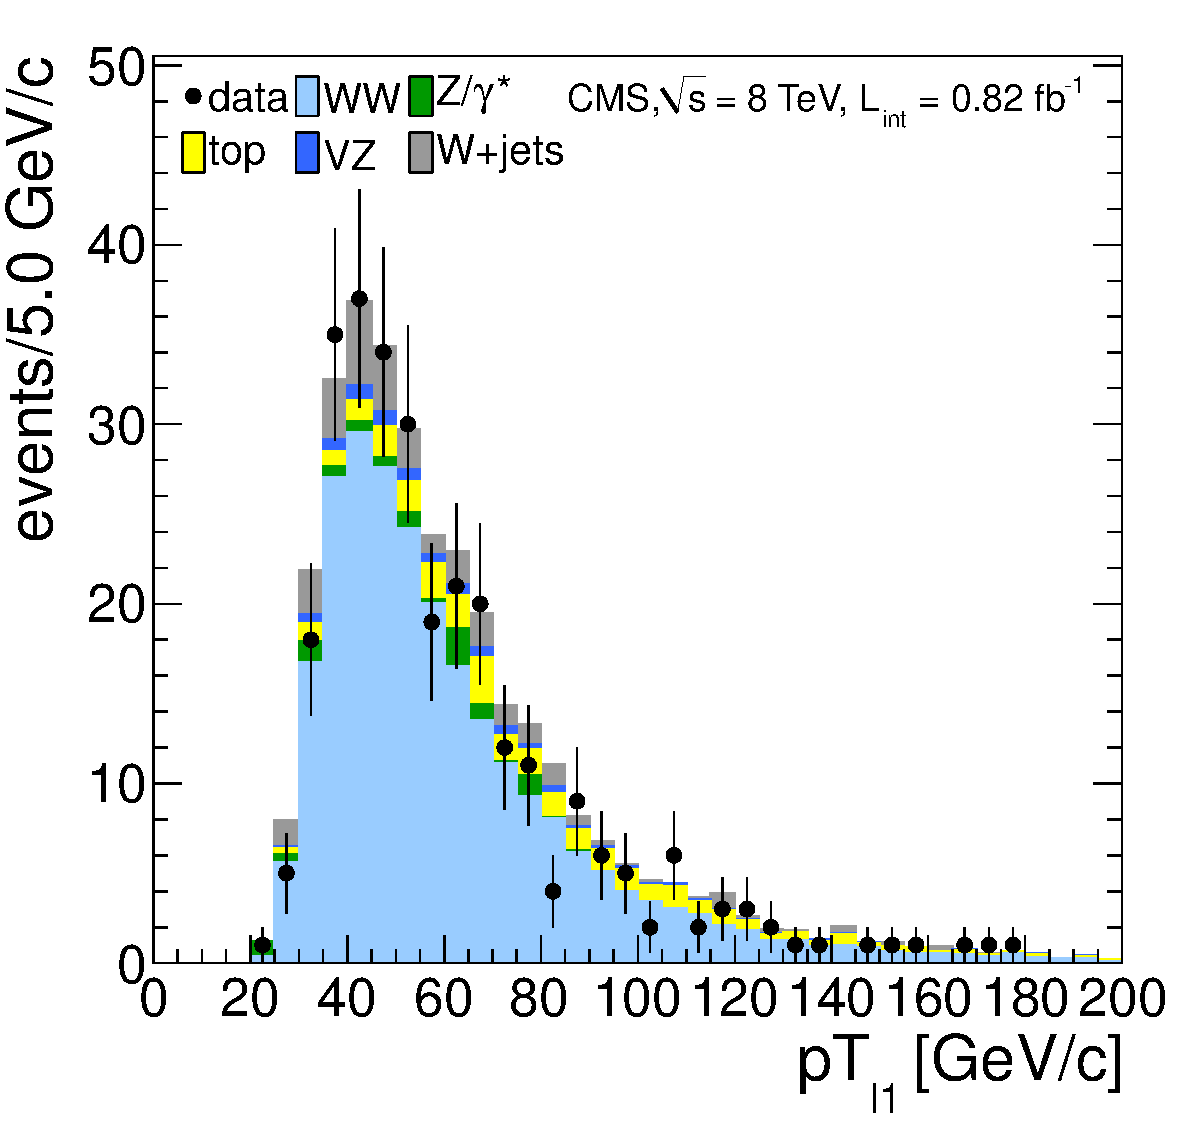
\includegraphics[width=.4\textwidth]{figures/lep1pt_mh0_nj0.pdf}
}
\subfigure[]{
\centering
\label{subfig:ww_ptmin_1j}
%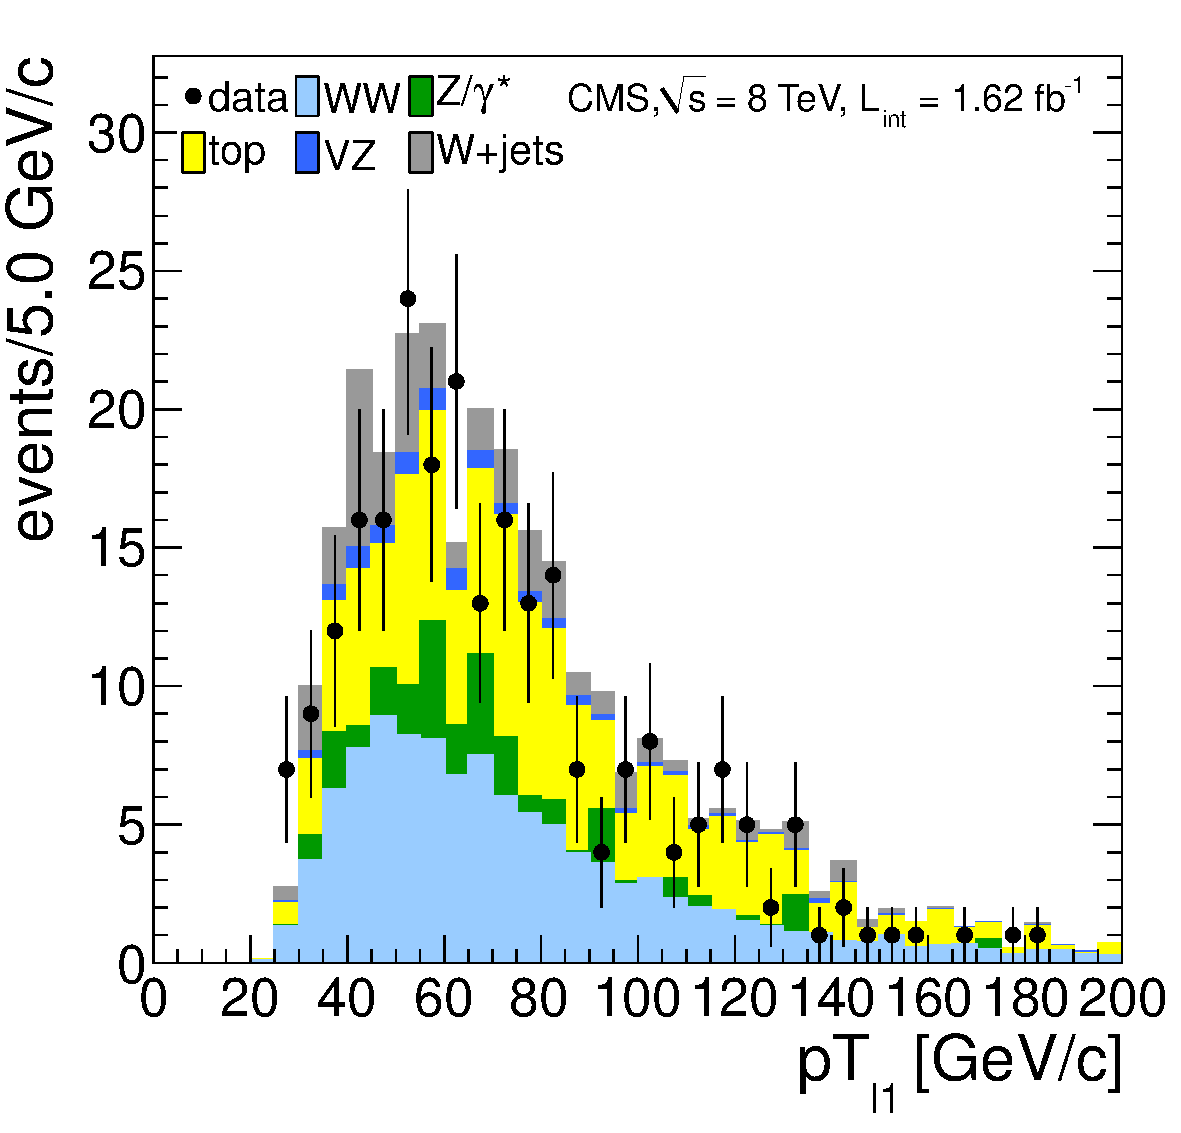
\includegraphics[width=.4\textwidth]{figures/lep1pt_mh0_nj1.pdf}
}
\subfigure[]{
\centering
\label{subfig:ww_ptmin_2j}
%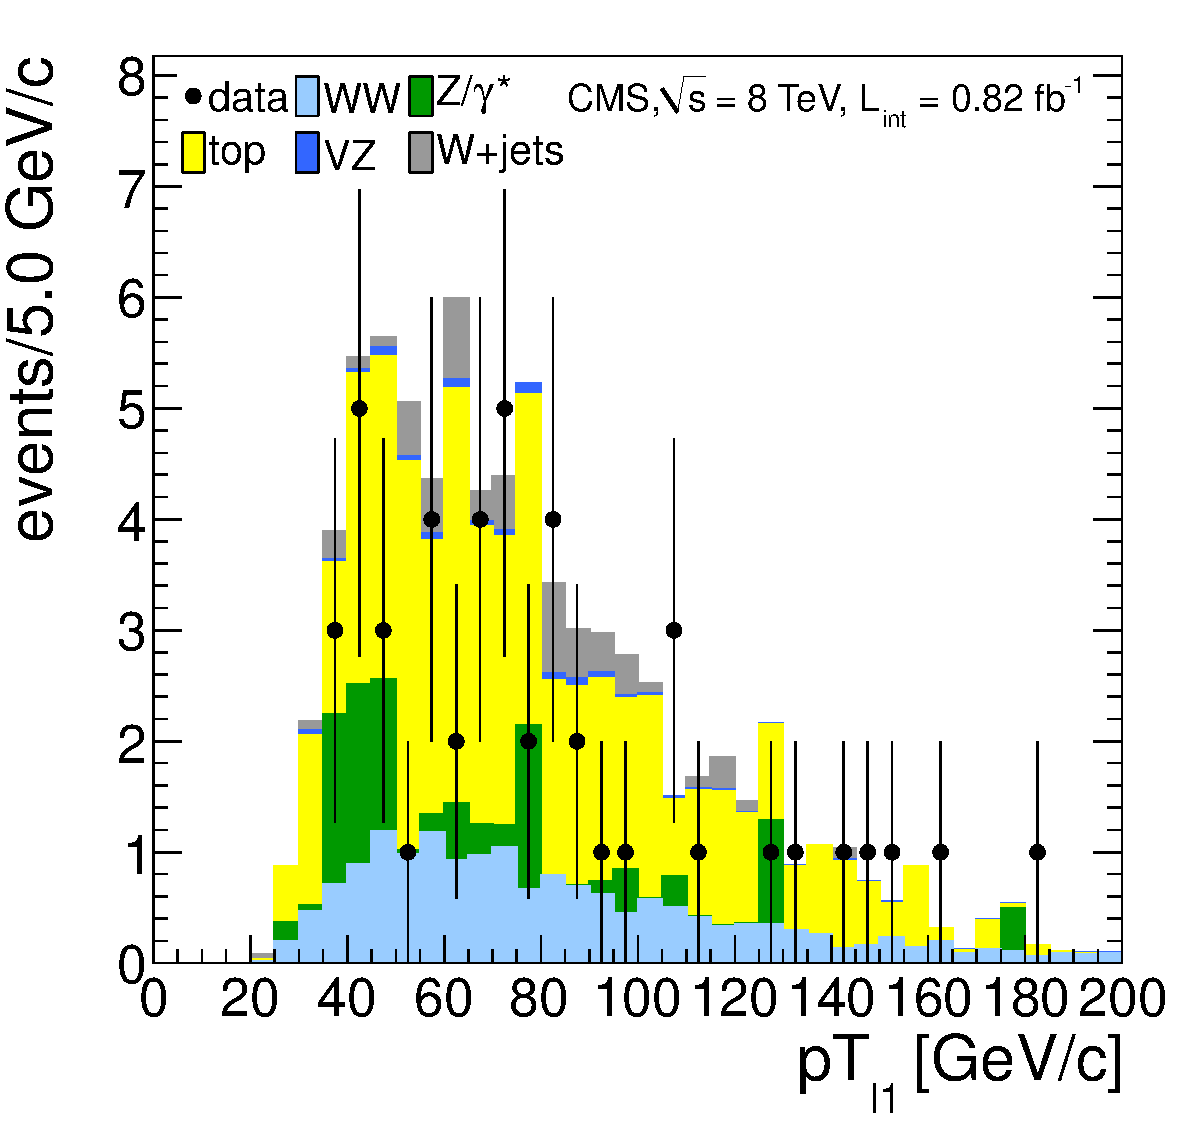
\includegraphics[width=.4\textwidth]{figures/lep1pt_mh0_nj2.pdf}
}
\caption{Trailing lepton $p_T$ distribution after WW selection for \intlumiEightTeV of data in the 0-jet \subref{subfig:ww_ptmin_0j}, 
1-jet \subref{subfig:ww_ptmin_1j} and 2-jet \subref{subfig:ww_ptmin_2j} bin analyses. 
MC is scaled to data-driven estimates.}
\label{fig:ww_ptmin}
\end{figure}

\begin{figure}[!hbtp]
\centering
\subfigure[]{
\centering
\label{subfig:ww_ptmax_0j}
%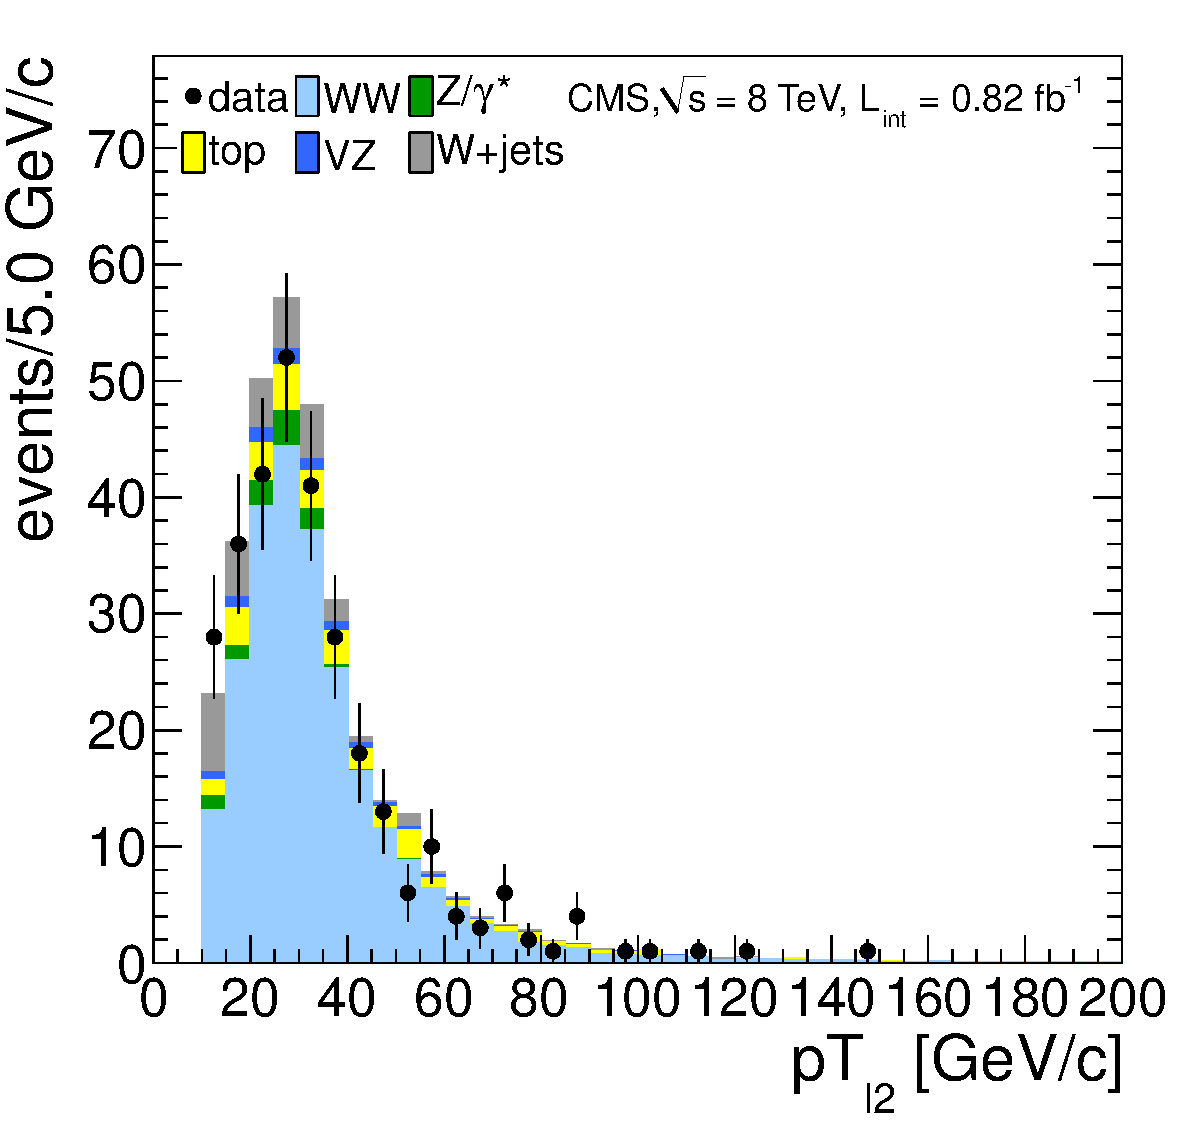
\includegraphics[width=.4\textwidth]{figures/lep2pt_mh0_nj0.pdf}
}
\subfigure[]{
\centering
\label{subfig:ww_ptmax_1j}
%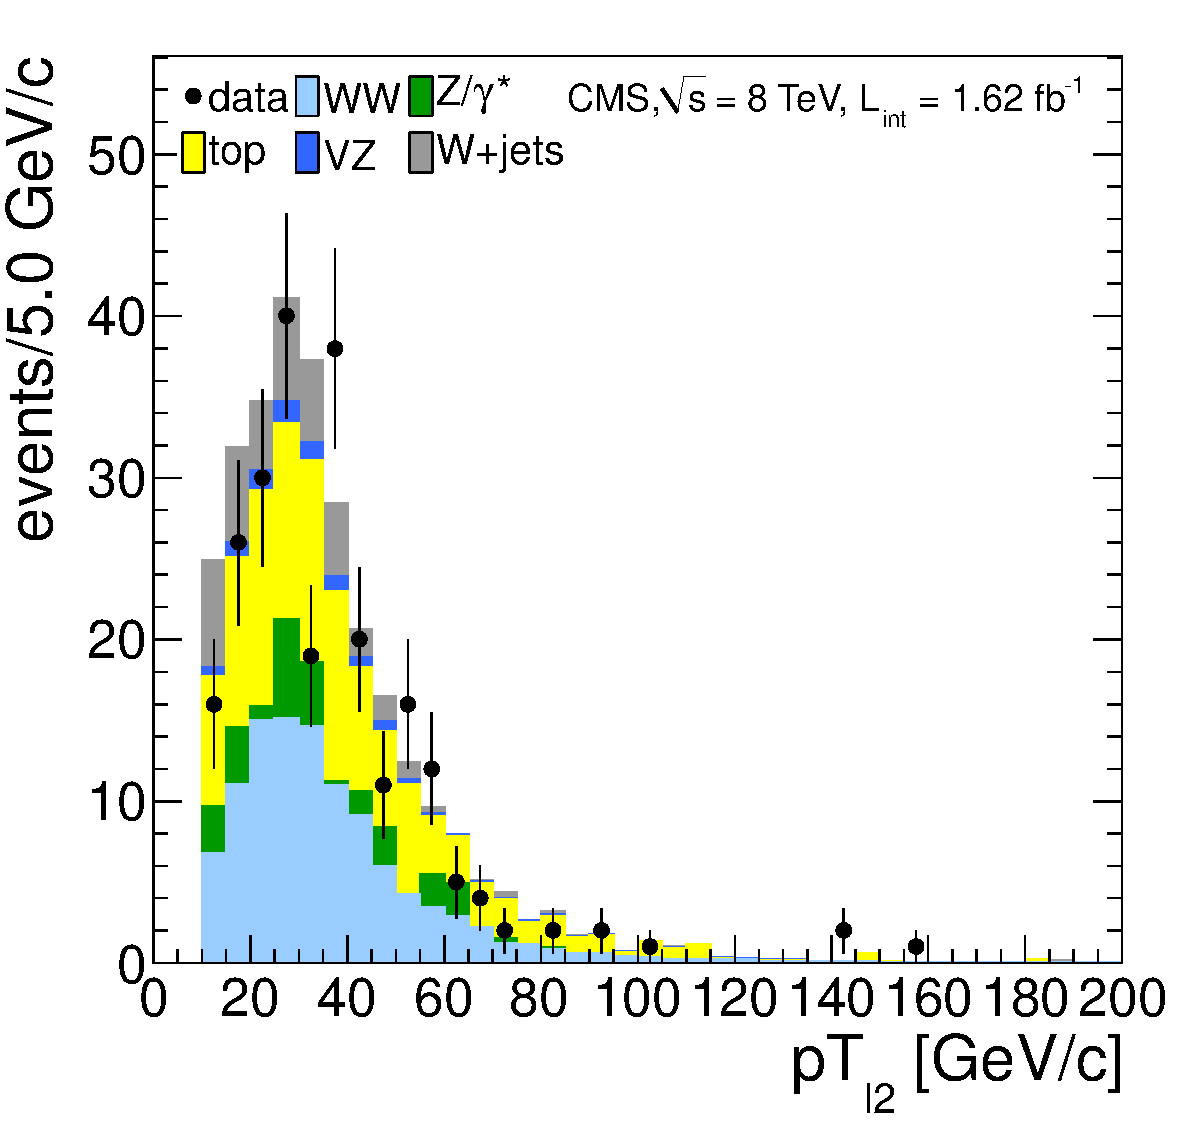
\includegraphics[width=.4\textwidth]{figures/lep2pt_mh0_nj1.pdf}
}
\subfigure[]{
\centering
\label{subfig:ww_ptmax_2j}
%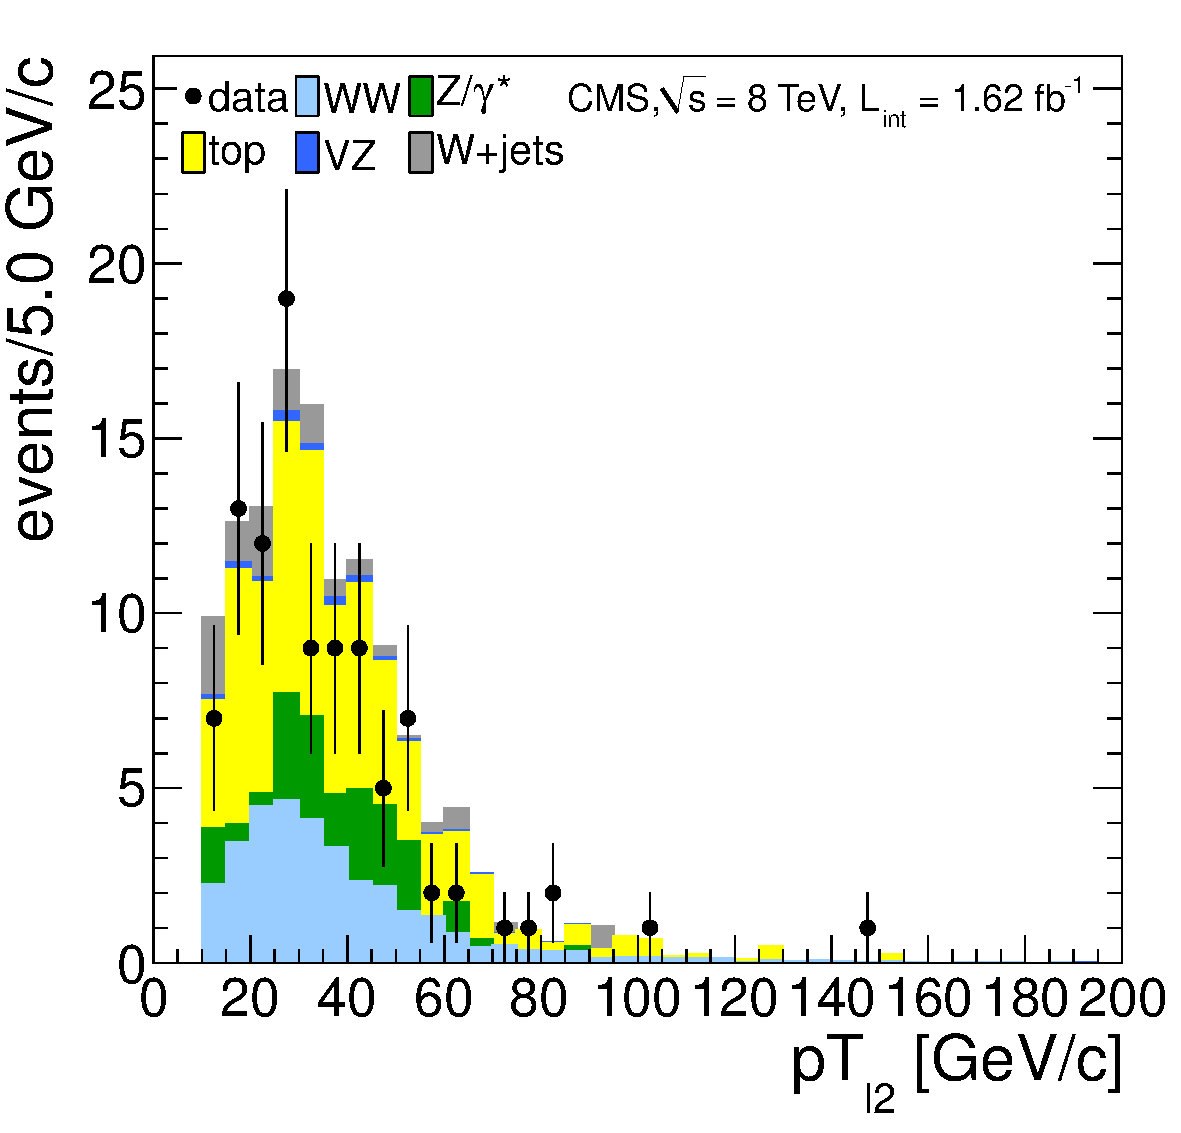
\includegraphics[width=.4\textwidth]{figures/lep2pt_mh0_nj2.pdf}
}\\
\caption{Leading lepton $p_T$ distribution after WW selection for \intlumiEightTeV of data in the 0-jet \subref{subfig:ww_ptmax_0j}, 
1-jet \subref{subfig:ww_ptmax_1j} and 2-jet \subref{subfig:ww_ptmax_2j} bin analyses. 
MC is scaled to data-driven estimates.}
\label{fig:ww_ptmax}
\end{figure}

\begin{figure}[!hbtp]
\centering
\subfigure[]{
\centering
\label{subfig:ww_pmet_0j}
%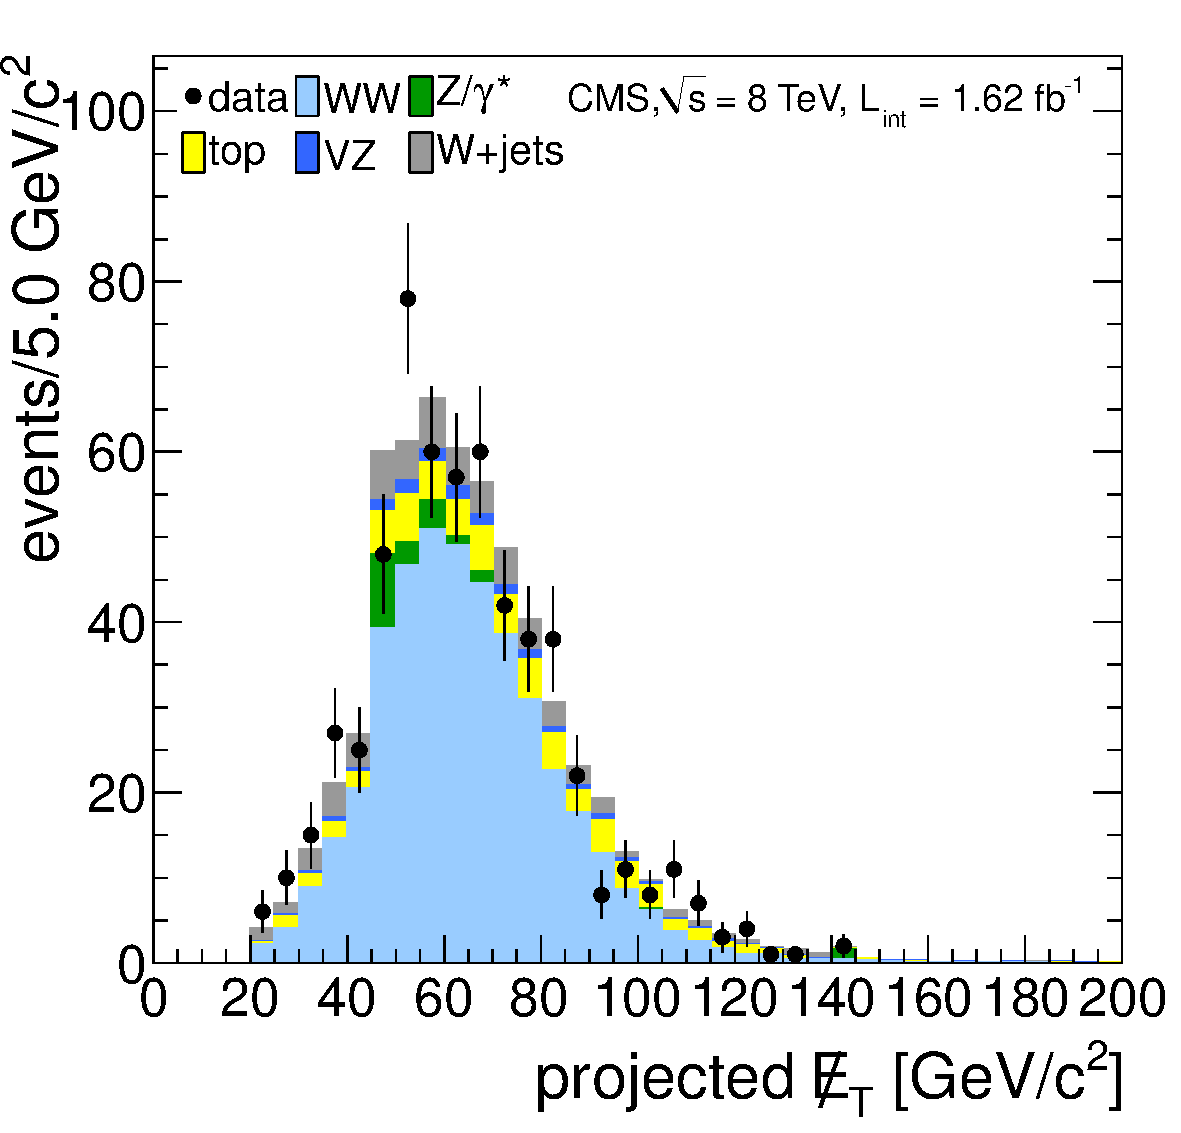
\includegraphics[width=.4\textwidth]{figures/pmet_mh0_nj0.pdf}
}
\subfigure[]{
\centering
\label{subfig:ww_pmet_1j}
%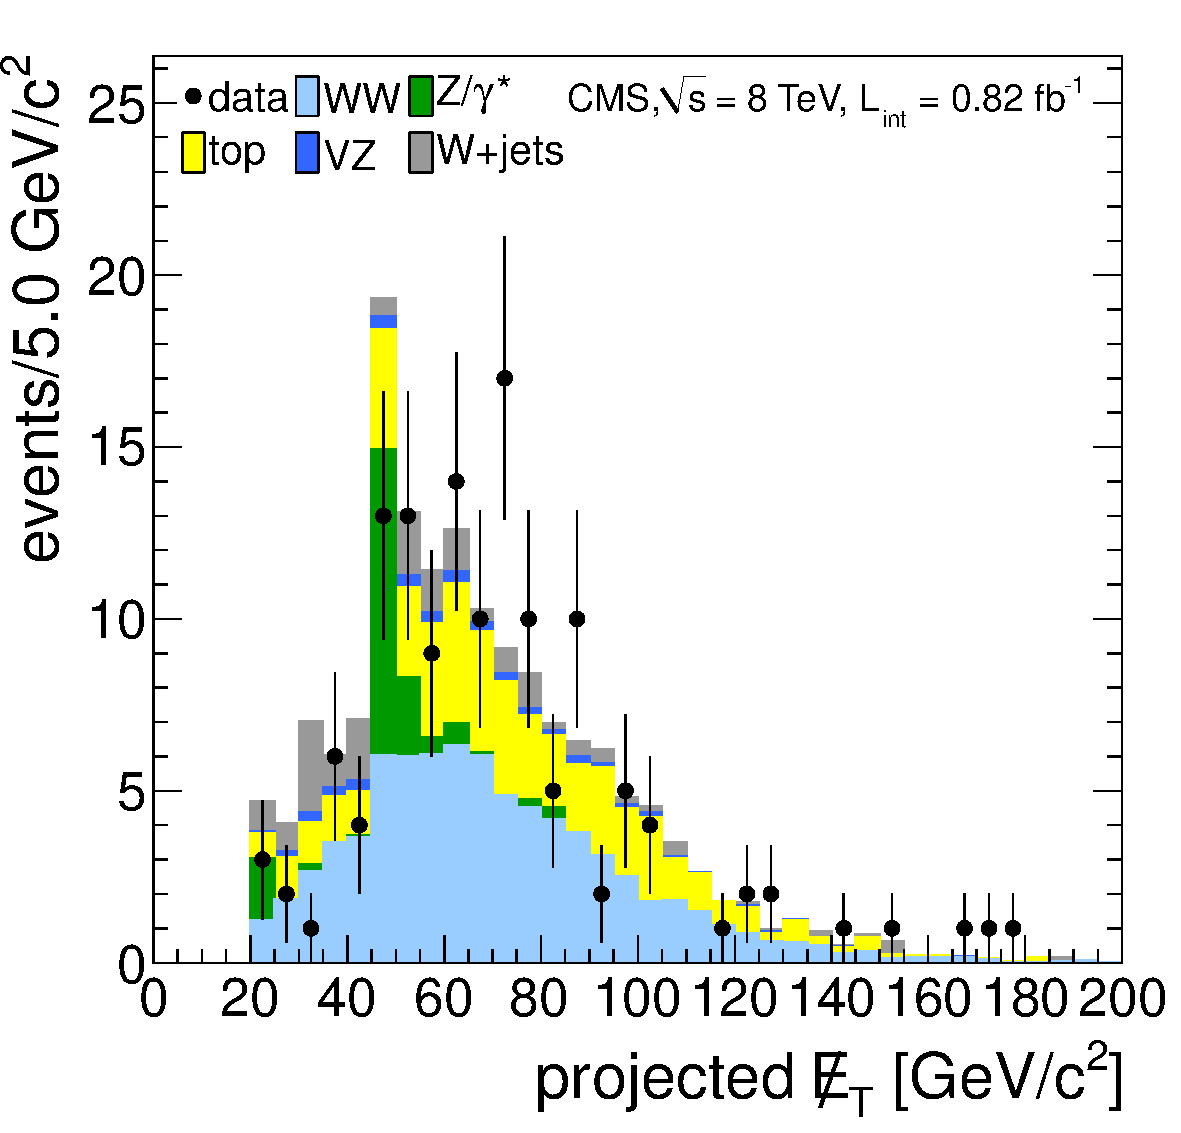
\includegraphics[width=.4\textwidth]{figures/pmet_mh0_nj1.pdf}
}
\subfigure[]{
\centering
\label{subfig:ww_pmet_2j}
%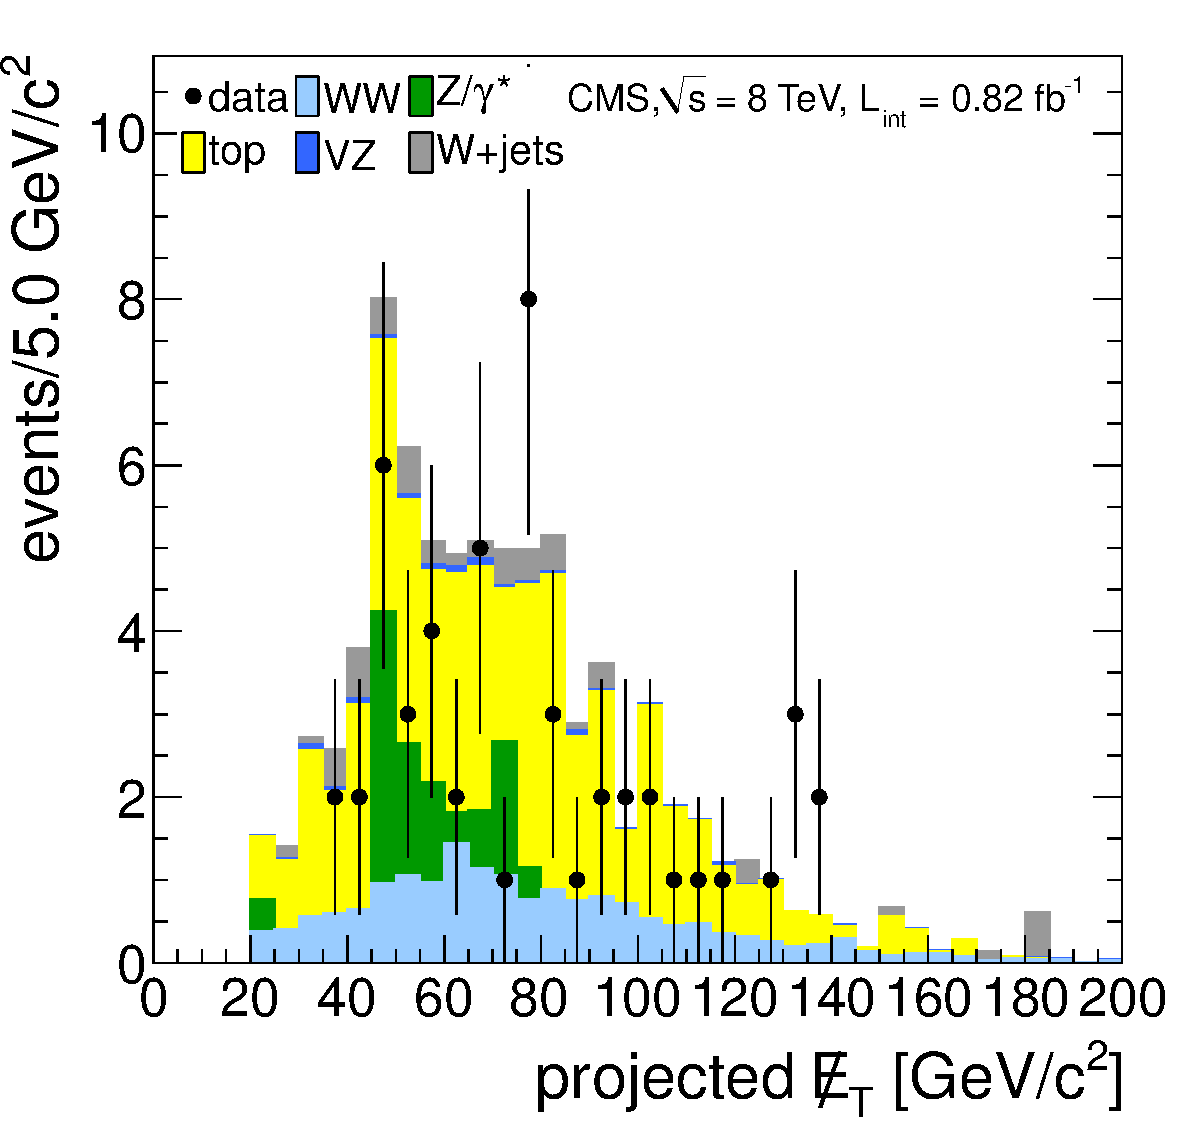
\includegraphics[width=.4\textwidth]{figures/pmet_mh0_nj2.pdf}
}\\
\caption{$min(\text{proj}_\text{trk-MET}, \text{proj}_\text{PFMET})$ distribution after WW selection for \intlumiEightTeV of data in the 0-jet \subref{subfig:ww_pmet_0j}, 
1-jet \subref{subfig:ww_pmet_1j} and 2-jet \subref{subfig:ww_pmet_2j} bin analyses. 
MC is scaled to data-driven estimates.}
\label{fig:ww_pmet}
\end{figure}

\begin{figure}[!hbtp]
\centering
\subfigure[]{
\centering
\label{subfig:ww_mt_0j}
%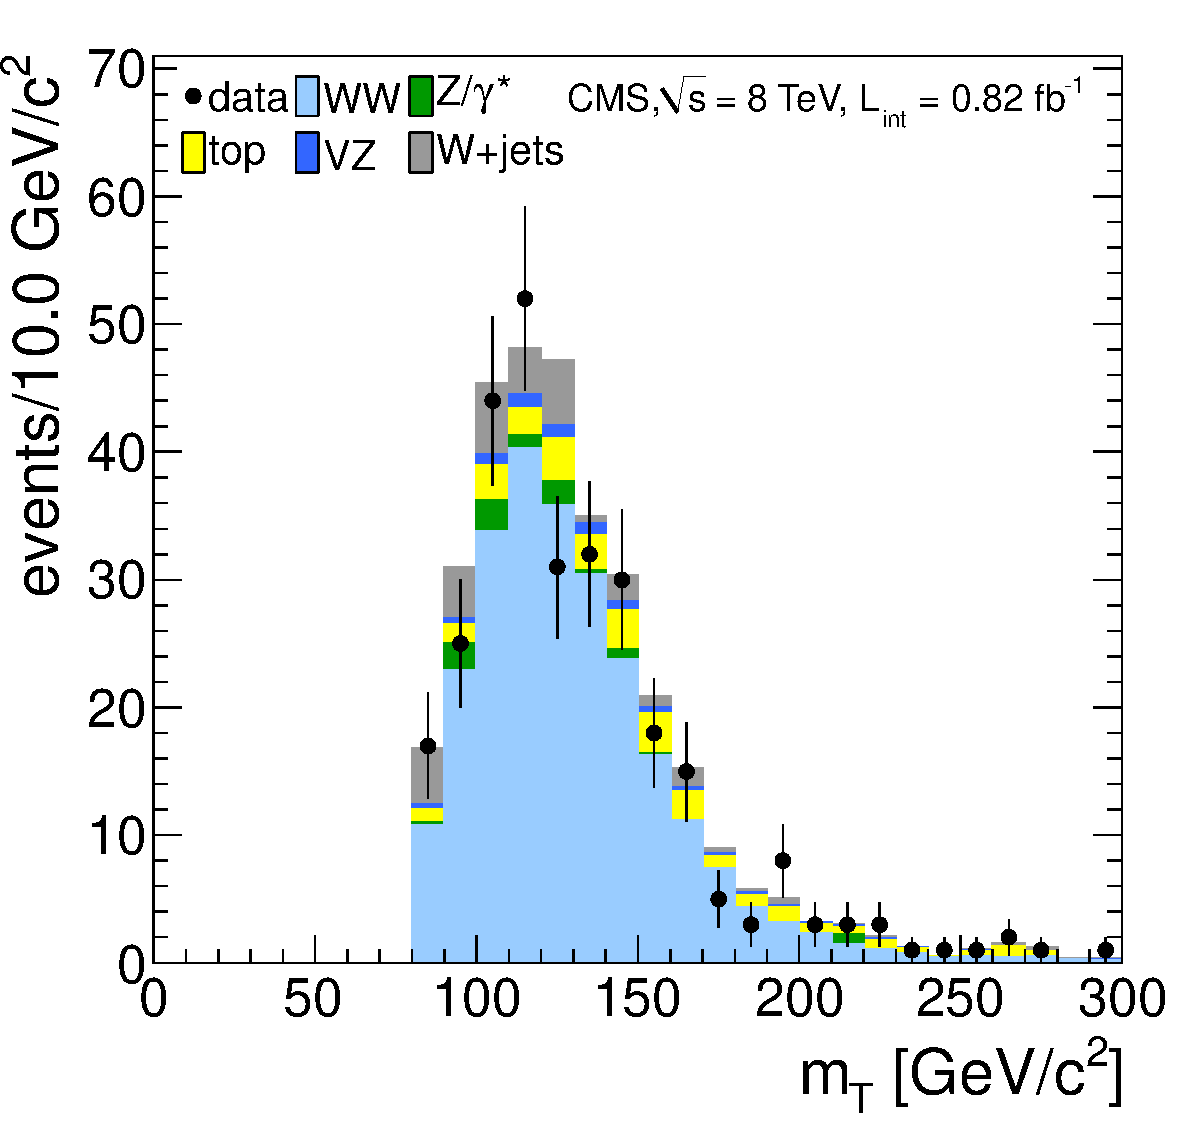
\includegraphics[width=.4\textwidth]{figures/mt_mh0_nj0.pdf}
}
\subfigure[]{
\centering
\label{subfig:ww_mt_1j}
%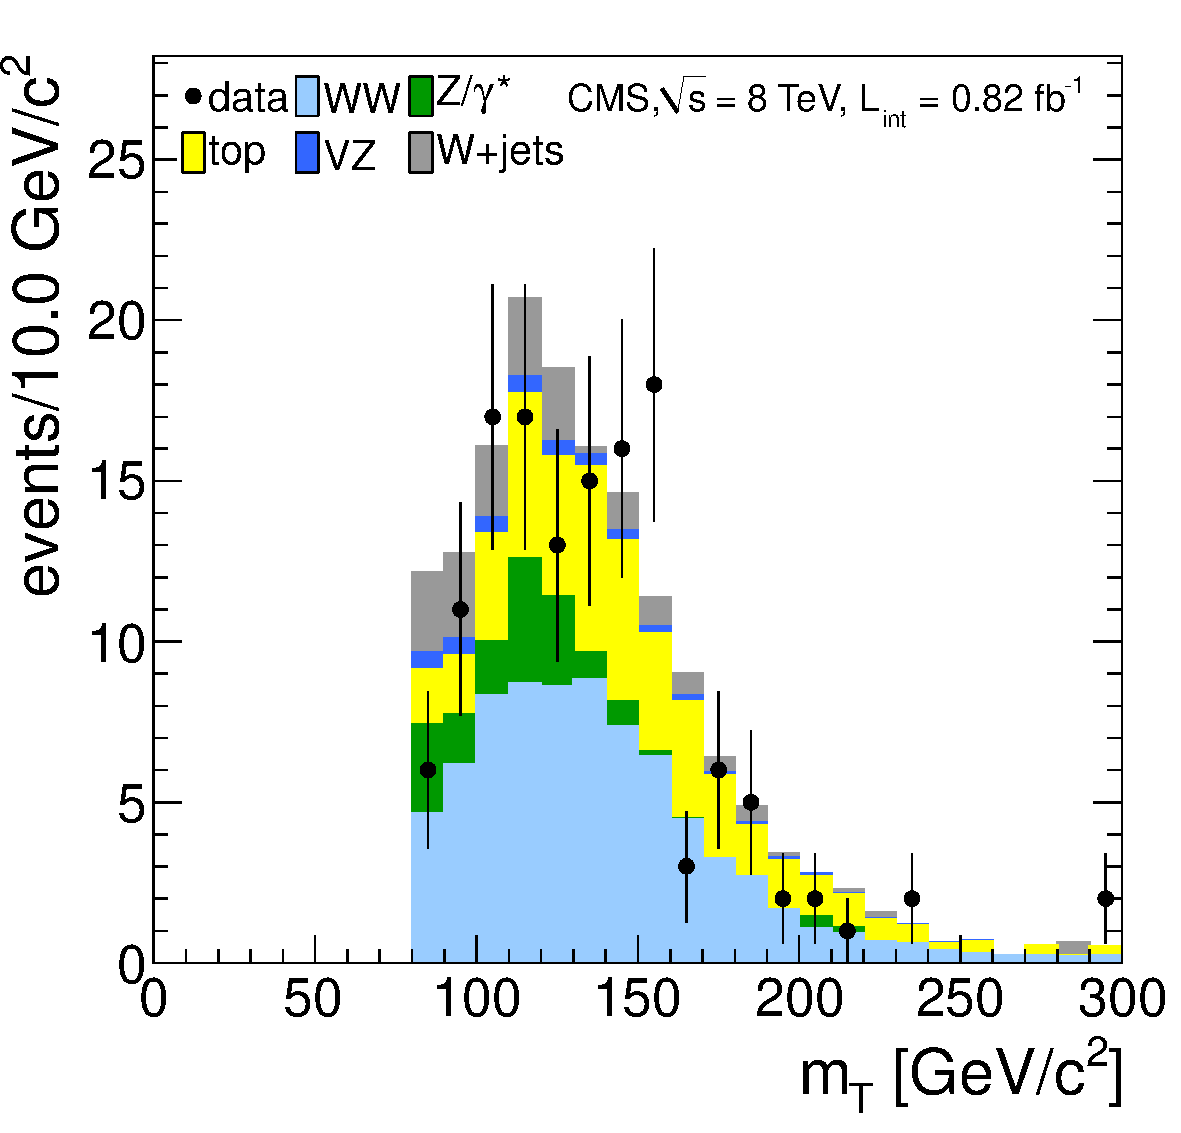
\includegraphics[width=.4\textwidth]{figures/mt_mh0_nj1.pdf}
}
\subfigure[]{
\centering
\label{subfig:ww_mt_2j}
%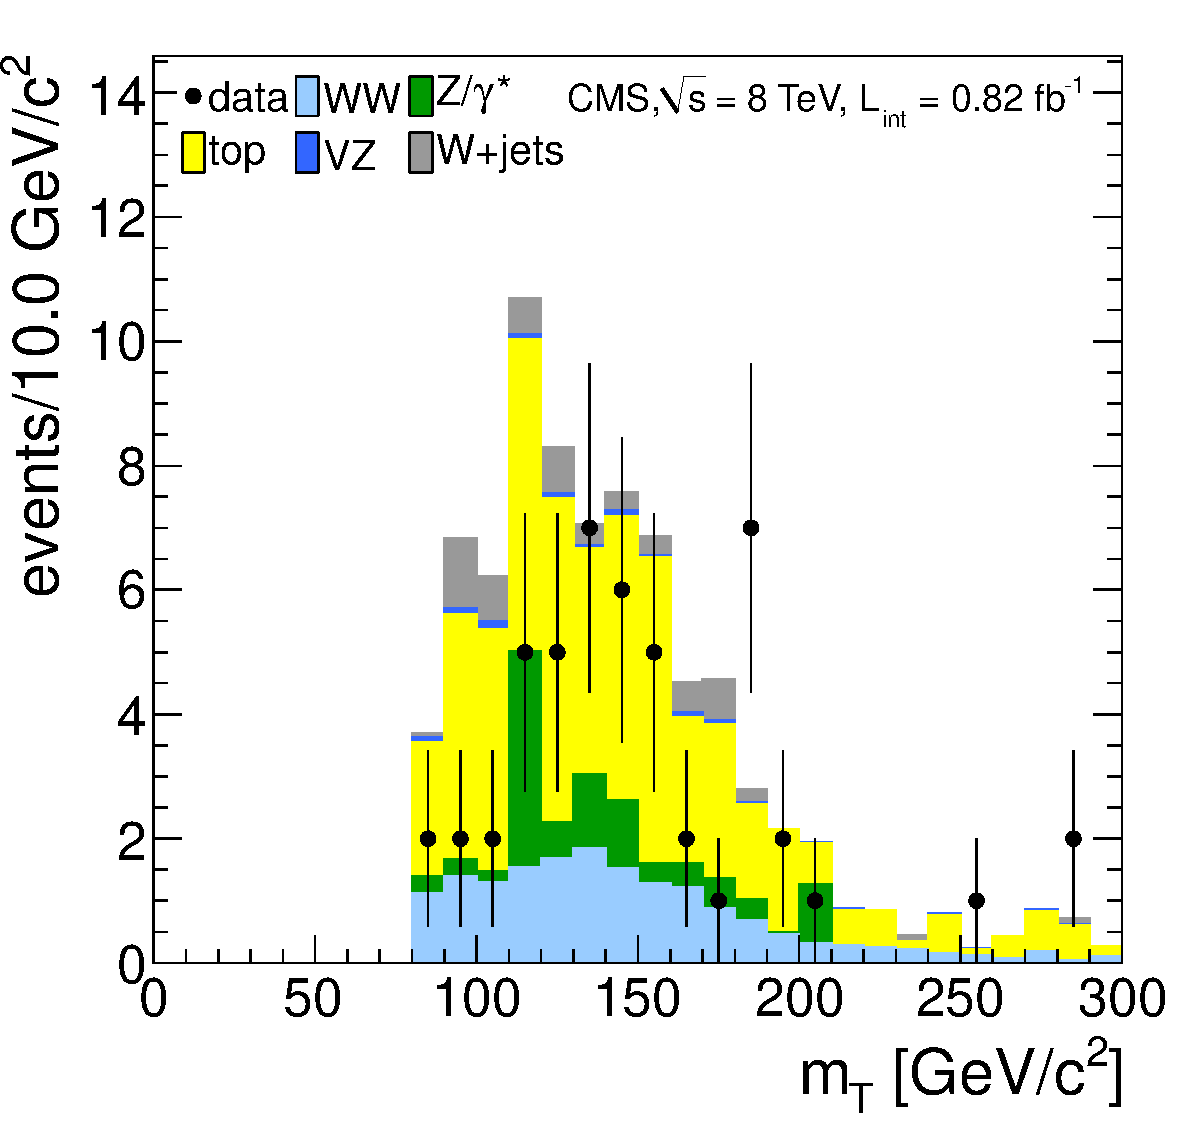
\includegraphics[width=.4\textwidth]{figures/mt_mh0_nj2.pdf}
} \\
\caption{Transverse mass distribution after WW selection for \intlumiEightTeV of data in the 0-jet \subref{subfig:ww_mt_0j}, 
1-jet \subref{subfig:ww_mt_1j} and 2-jet \subref{subfig:ww_mt_2j} bin analyses. 
MC is scaled to data-driven estimates.}
\label{fig:ww_mt}
\end{figure}

\begin{figure}[!hbtp]
\centering
\subfigure[]{
\centering
\label{subfig:ww_dilmass_0j}
%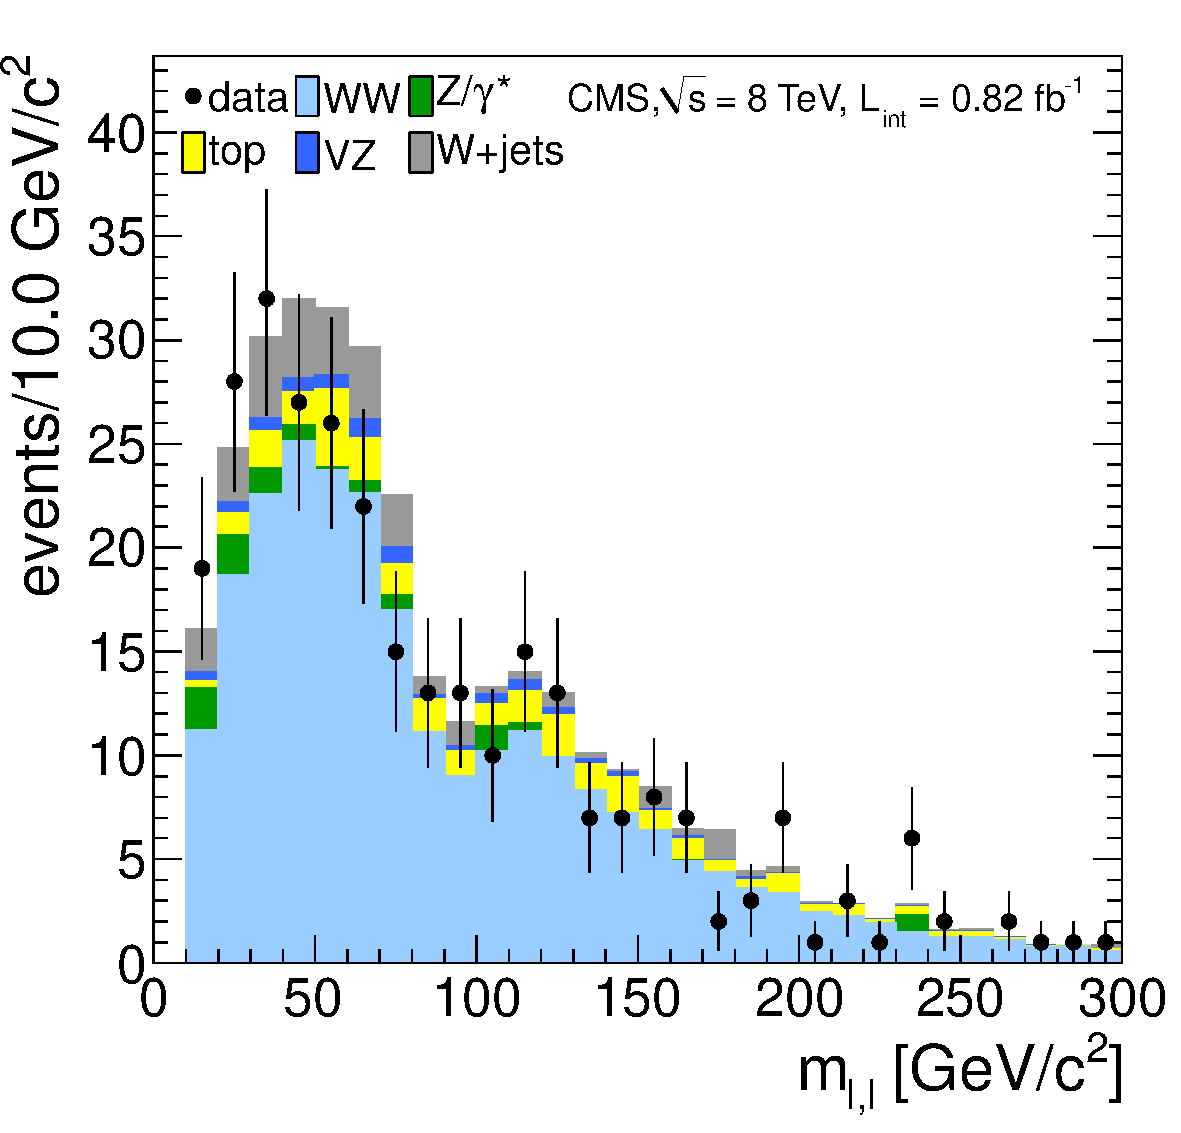
\includegraphics[width=.4\textwidth]{figures/dilepmass_mh0_nj0.pdf}
}
\subfigure[]{
\centering
\label{subfig:ww_dilmass_1j}
%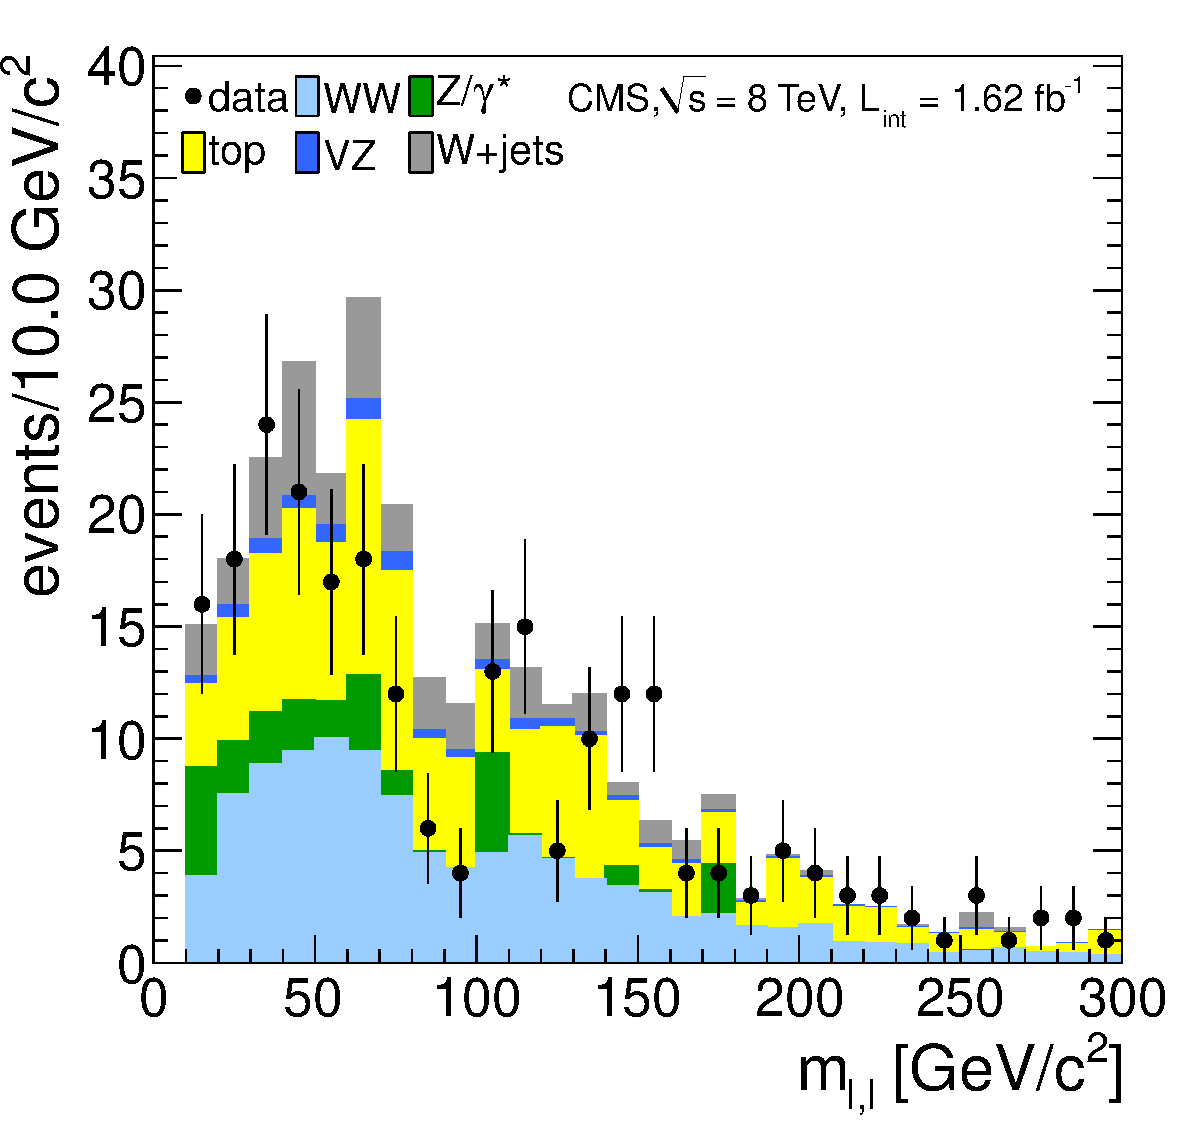
\includegraphics[width=.4\textwidth]{figures/dilepmass_mh0_nj1.pdf}
}
\subfigure[]{
\centering
\label{subfig:ww_dilmass_2j}
%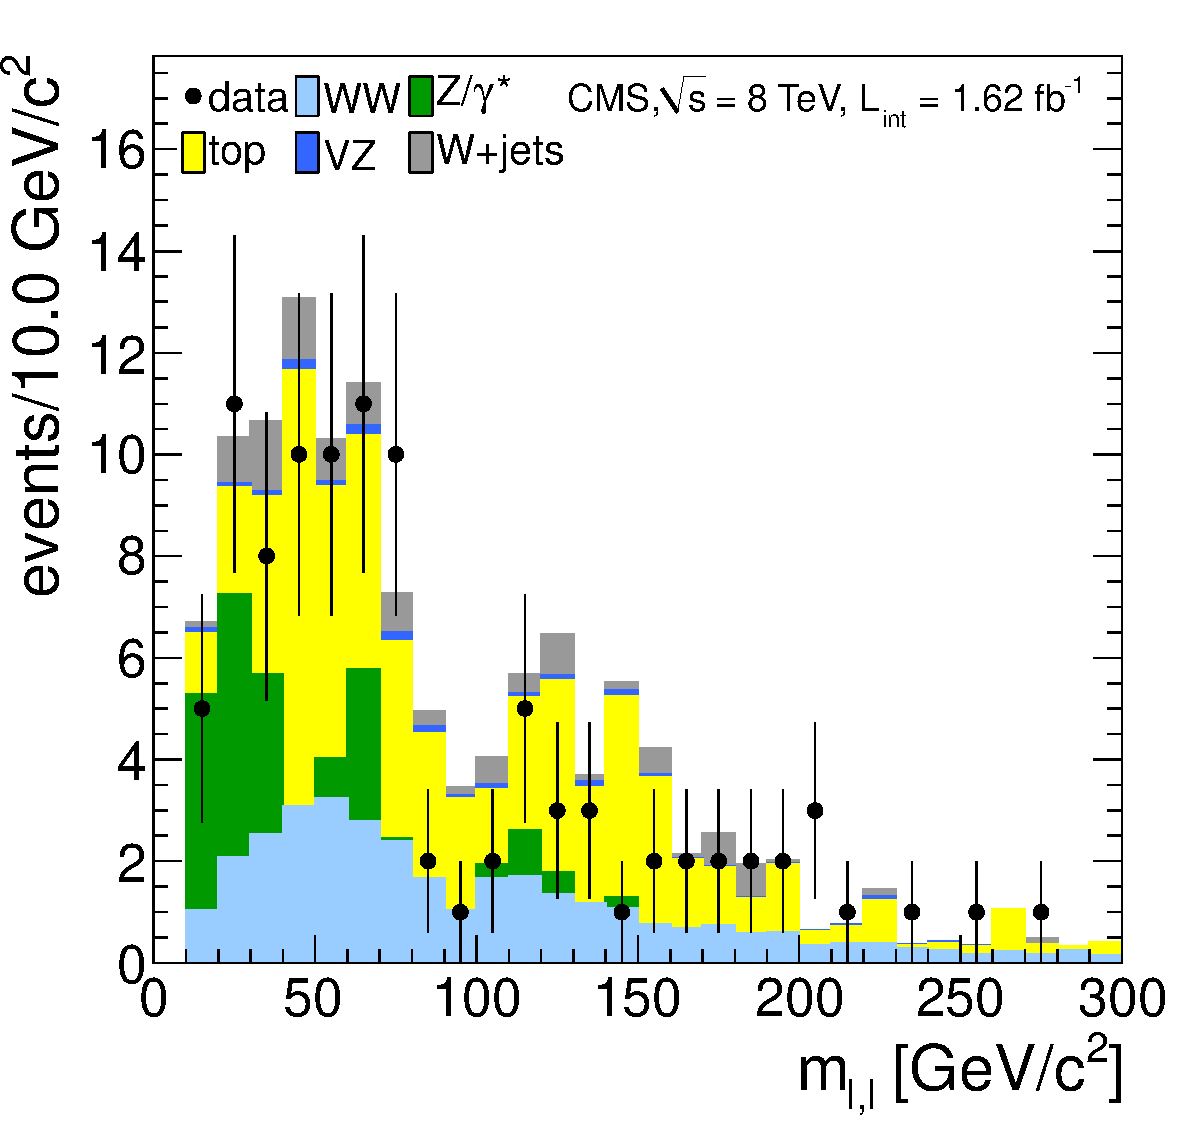
\includegraphics[width=.4\textwidth]{figures/dilepmass_mh0_nj2.pdf}
} \\
\caption{Invariant dilepton mass distribution after WW selection for \intlumiEightTeV of data in the 0-jet \subref{subfig:ww_dilmass_0j}, 
1-jet \subref{subfig:ww_dilmass_1j} and 2-jet \subref{subfig:ww_dilmass_2j} bin analyses. 
MC is scaled to data-driven estimates.}
\label{fig:ww_dilmass}
\end{figure}

\begin{figure}[!hbtp]
\centering
\subfigure[]{
\centering
\label{subfig:ww_deltaphi_0j}
%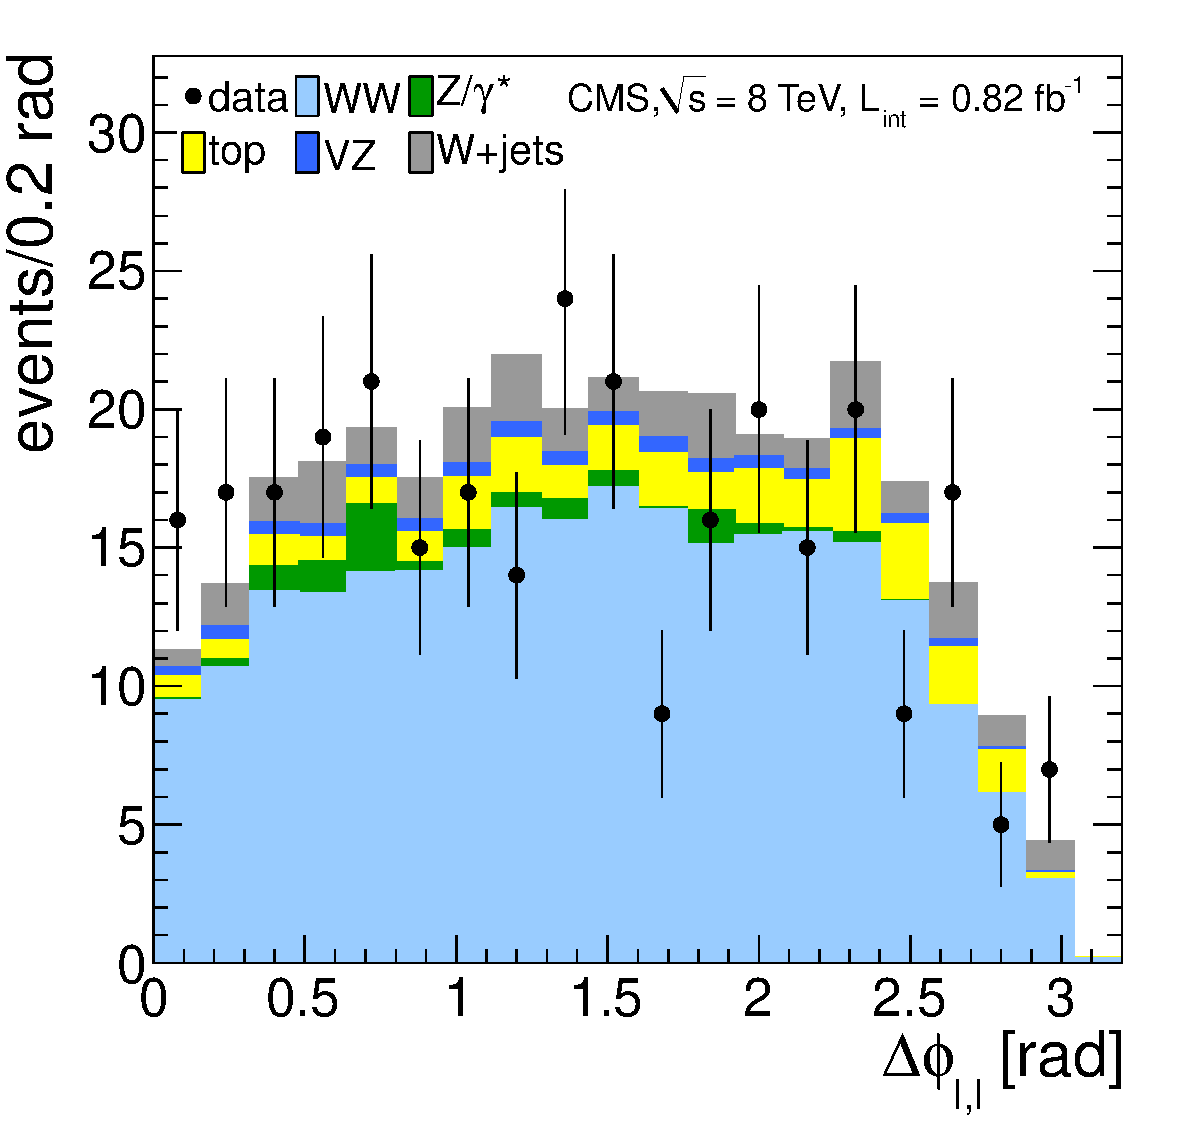
\includegraphics[width=.4\textwidth]{figures/dPhi_mh0_nj0.pdf}
}
\subfigure[]{
\centering
\label{subfig:ww_deltaphi_1j}
%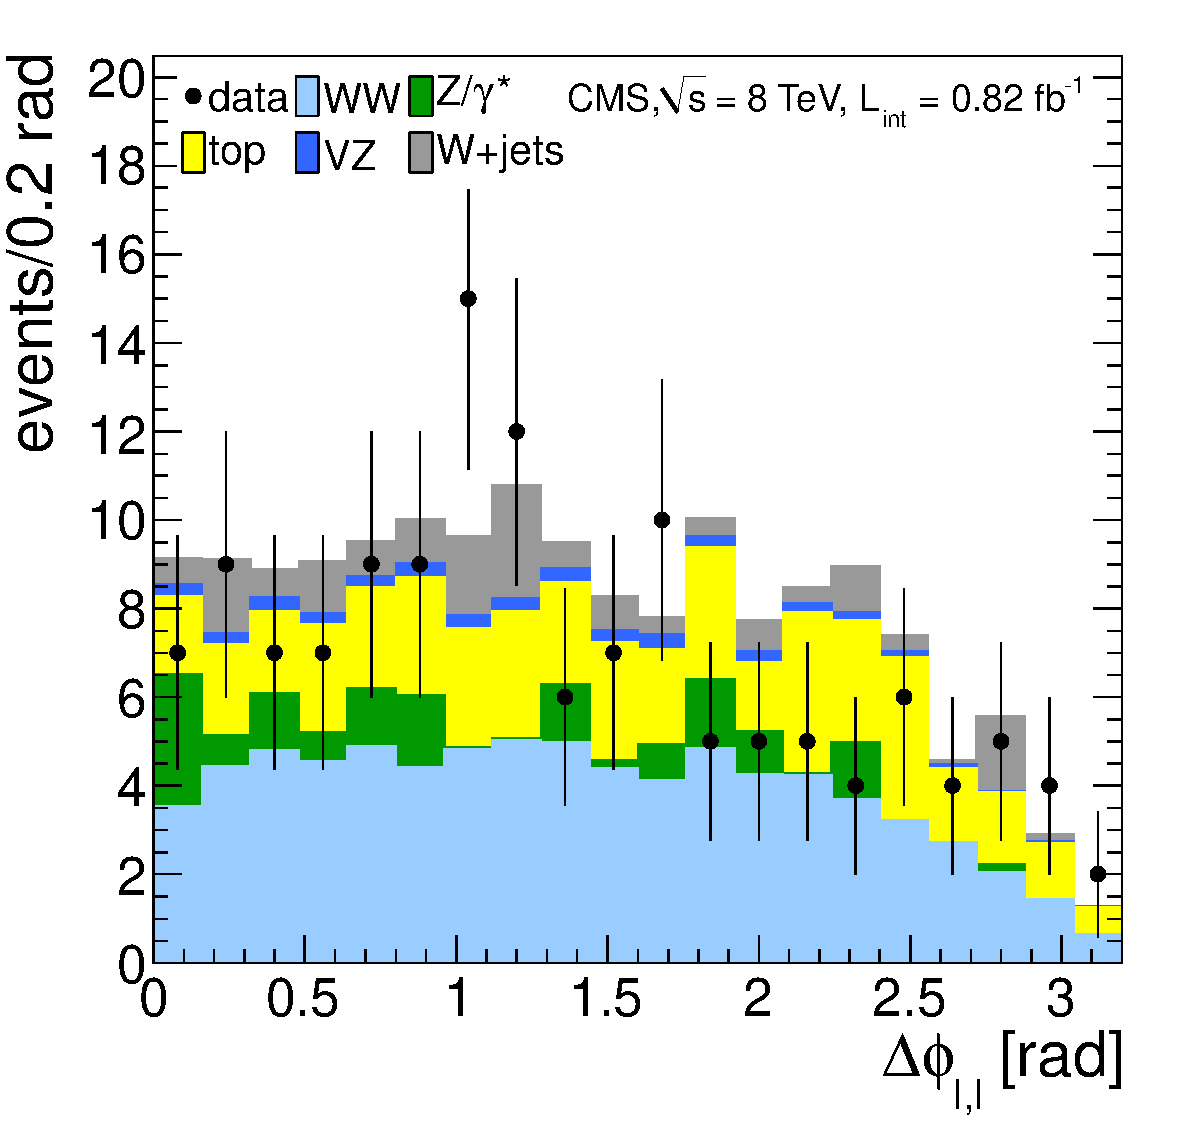
\includegraphics[width=.4\textwidth]{figures/dPhi_mh0_nj1.pdf}
}
\subfigure[]{
\centering
\label{subfig:ww_deltaphi_2j}
%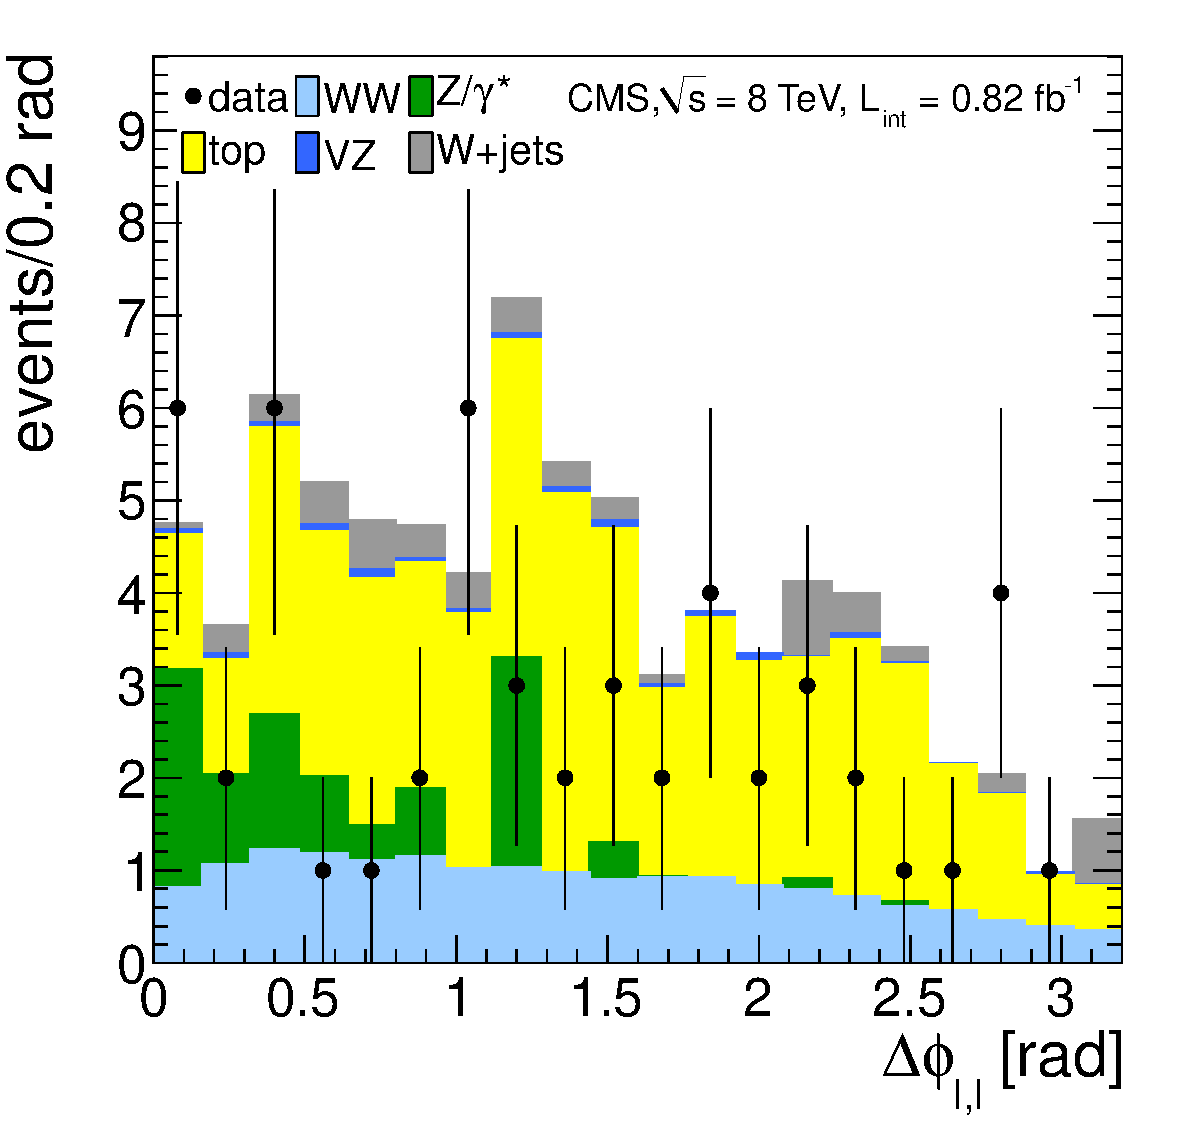
\includegraphics[width=.4\textwidth]{figures/dPhi_mh0_nj2.pdf}
} \\
\caption{Dilepton $\Delta\phi$ distribution after WW selection for \intlumiEightTeV of data in the 0-jet \subref{subfig:ww_deltaphi_0j}, 
1-jet \subref{subfig:ww_deltaphi_1j} and 2-jet \subref{subfig:ww_deltaphi_2j} bin analyses. 
MC is scaled to data-driven estimates.}
\label{fig:ww_deltaphi}
\end{figure}

\clearpage


\begin{table}[ht!]
\begin{center}
\begin{tabular}{c | c c c | c c c} 
\hline
              & \multicolumn{3}{c|}{0-jet} & \multicolumn{3}{c}{1-jet} \\
mass [\GeVcc] & data estimate & MC prediction & scale factor & data estimate & MC prediction & scale factor \\
\hline
115 &  68.1 $\pm$  5.5 &  59.5 $\pm$  1.0 & 1.14 $\pm$ 0.10 &  21.1 $\pm$  3.1 &  16.9 $\pm$  0.6 & 1.25 $\pm$ 0.19 \\
120 & 102.3 $\pm$  8.3 &  89.4 $\pm$  1.3 & 1.14 $\pm$ 0.09 &  29.8 $\pm$  4.4 &  23.9 $\pm$  0.7 & 1.25 $\pm$ 0.19 \\
130 & 143.3 $\pm$ 11.5 & 125.3 $\pm$  1.5 & 1.14 $\pm$ 0.09 &  42.3 $\pm$  6.2 &  33.9 $\pm$  0.8 & 1.25 $\pm$ 0.19 \\
140 & 151.1 $\pm$ 12.0 & 131.3 $\pm$  1.5 & 1.15 $\pm$ 0.09 &  44.7 $\pm$  6.3 &  34.8 $\pm$  0.8 & 1.28 $\pm$ 0.18 \\
150 & 117.8 $\pm$  9.8 & 103.4 $\pm$  1.4 & 1.14 $\pm$ 0.10 &  43.7 $\pm$  6.5 &  34.0 $\pm$  0.8 & 1.29 $\pm$ 0.19 \\
160 &  83.6 $\pm$  7.0 &  73.2 $\pm$  1.1 & 1.14 $\pm$ 0.10 &  36.9 $\pm$  5.5 &  28.7 $\pm$  0.7 & 1.29 $\pm$ 0.19 \\
170 &  66.9 $\pm$  5.6 &  58.6 $\pm$  1.0 & 1.14 $\pm$ 0.10 &  31.3 $\pm$  4.6 &  24.1 $\pm$  0.7 & 1.30 $\pm$ 0.20 \\
180 &  79.2 $\pm$  6.6 &  69.7 $\pm$  1.1 & 1.14 $\pm$ 0.10 &  37.8 $\pm$  5.6 &  29.2 $\pm$  0.7 & 1.29 $\pm$ 0.19 \\
190 & 122.1 $\pm$ 10.2 & 107.6 $\pm$  1.4 & 1.13 $\pm$ 0.10 &  59.6 $\pm$  8.8 &  46.1 $\pm$  0.9 & 1.29 $\pm$ 0.19 \\
\hline
\end{tabular}
\caption{WW background estimation for $\intlumiEightTeV$.}
\label{tab:ww_est}
\end{center}
\end{table}

\begin{figure}[!hbtp]
\centering
\subfigure[]{
\centering
\label{subfig:ww_dilmass_0j_nozveto}
%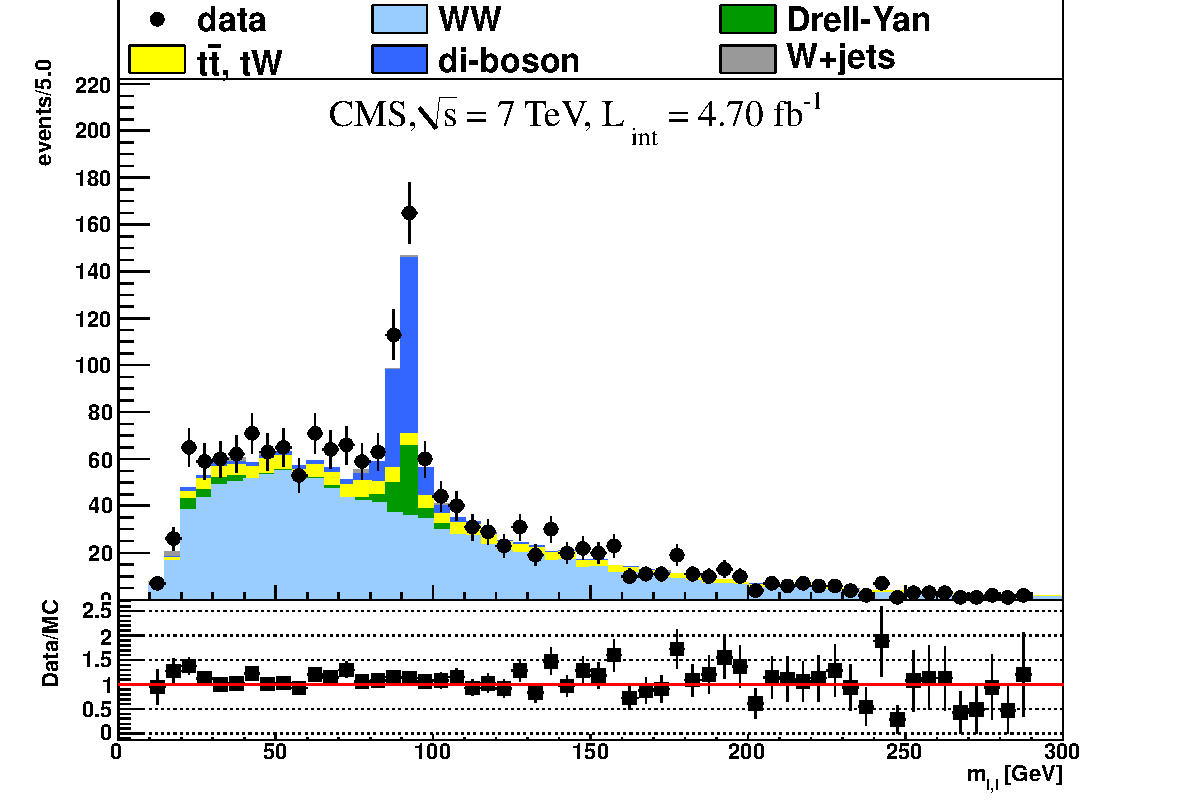
\includegraphics[width=.4\textwidth]{figures/dilepmass_mh0_nj0_nozveto.pdf}
}
\subfigure[]{
\centering
\label{subfig:ww_dilmass_1j_nozveto}
%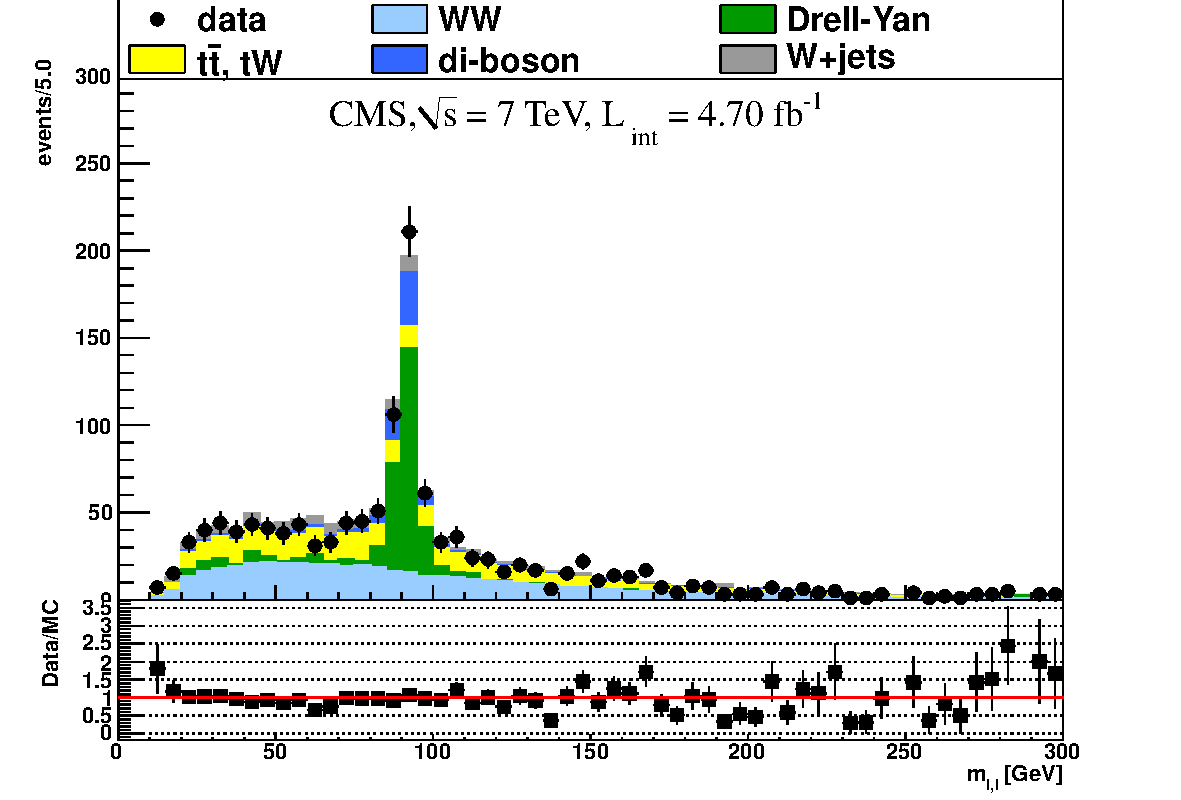
\includegraphics[width=.4\textwidth]{figures/dilepmass_mh0_nj1_nozveto.pdf}
}
\subfigure[]{
\centering
\label{subfig:ww_dilmass_2j_nozveto}
%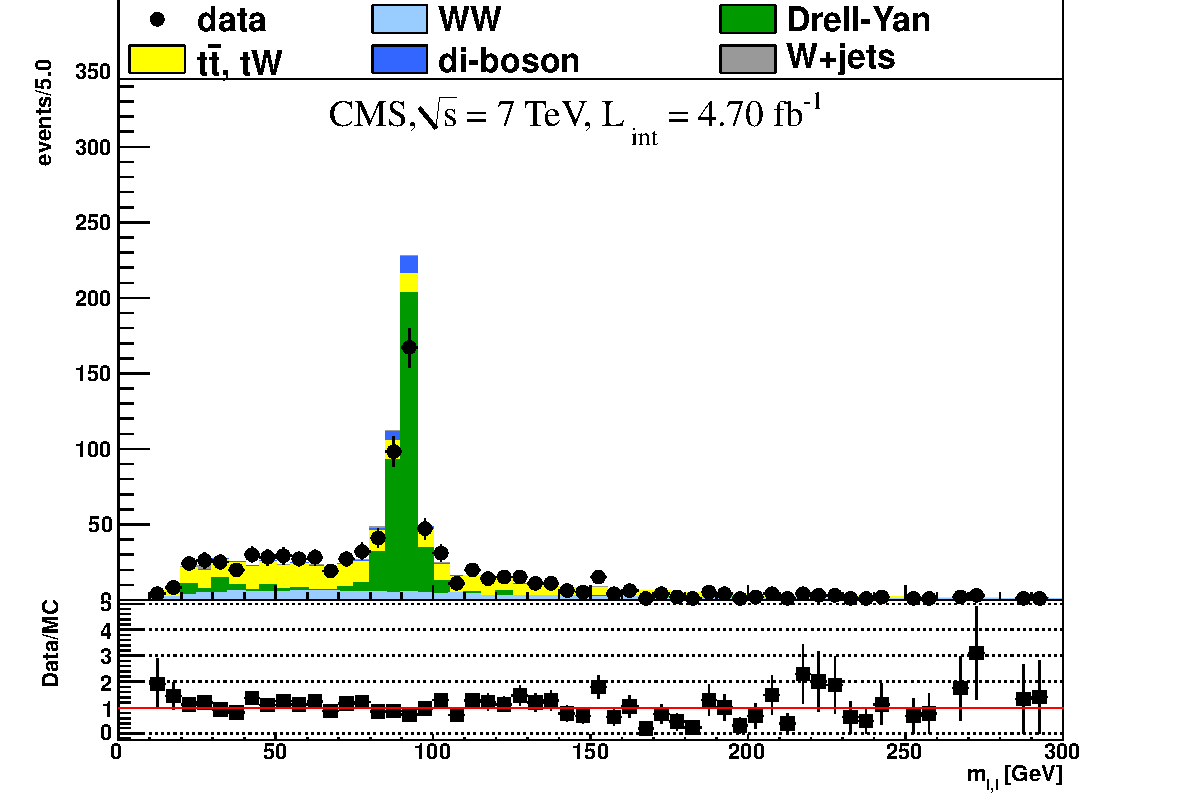
\includegraphics[width=.4\textwidth]{figures/dilepmass_mh0_nj2_nozveto.pdf}
} \\
\caption{Invariant dilepton mass distribution after WW selection wihtou applying the Z veto for 
\intlumiEightTeV of data in the 0-jet \subref{subfig:ww_dilmass_0j_nozveto}, 
1-jet \subref{subfig:ww_dilmass_1j_nozveto} and 2-jet \subref{subfig:ww_dilmass_2j_nozveto} bin analyses. 
MC is scaled to data-driven estimates. In the 2-jet bin, the difference between data and MC under the Z peak is 
covered by the unceratinty on the scale factor.}
\label{fig:ww_dilmass_nozveto}
\end{figure}

%%%%%%%%%%%%%%%%%%%%%%%%%%%%%%
\begin{table}[!hbp]
\begin{center}
\begin{tabular}{c c c c c c}
\hline
\vspace{-3mm} && \\
 Selection [\GeVcc] &  Region   &  MC Yield & MC effic. [\%] & Data Yield & Data effic. [\%] \\
\vspace{-3mm} && \\
\hline
\multirow{3}{*}{$m_H$=120} & ww sideband  & 317.1 $\pm$   2.4 &  -  &  380.3 $\pm$  27.8 &  - \\
                                  & + 70$<m_T<$120  & 138.3 $\pm$   1.6 &   43.6 $\pm$   0.4 & 168.6 $\pm$  16.4 &   44.3 $\pm$   2.5 \\
                           & + $\Delta\phi<$115  &  37.2 $\pm$   0.8 &   26.9 $\pm$   0.5 & 60.8 $\pm$   9.4 &   36.0 $\pm$   3.7 \\
\hline
\multirow{3}{*}{$m_H$=130} & ww sideband  &  317.1 $\pm$   2.4 &  - & 380.3 $\pm$  27.8 &  - \\                                 
                                   & + 75$<m_T<$125  &  156.9 $\pm$   1.7 &   49.5 $\pm$   0.4 & 180.3 $\pm$  17.6 &   47.4 $\pm$   2.6 \\
                            & + $\Delta\phi<$90  &   17.7 $\pm$   0.6 &   11.3 $\pm$   0.3 &  16.5 $\pm$   7.3 &    9.2 $\pm$   2.1 \\
\hline                                                                                                                                
\multirow{3}{*}{$m_H$=140} & ww sideband  &  314.6 $\pm$   2.4 &  - & 379.5 $\pm$  27.5 &  - \\                                
                                   & + 80$<m_T<$130  &  171.5 $\pm$   1.8 &   54.5 $\pm$   0.4 & 197.7 $\pm$  18.4 &   52.1 $\pm$   2.6 \\
                            & + $\Delta\phi<$90  &   21.3 $\pm$   0.6 &   12.4 $\pm$   0.3 &  20.5 $\pm$   7.1 &   10.4 $\pm$   2.2 \\
\hline                                                                                                                                
\multirow{3}{*}{$m_H$=150} & ww sideband  &  284.9 $\pm$   2.3 &  - & 337.8 $\pm$  26.0 &  - \\                                
                                   & + 80$<m_T<$150  &  211.5 $\pm$   2.0 &   74.2 $\pm$   0.4 & 256.0 $\pm$  20.0 &   75.8 $\pm$   2.3 \\
                            & + $\Delta\phi<$90  &   25.1 $\pm$   0.7 &   11.9 $\pm$   0.3 &  29.4 $\pm$   6.4 &   11.5 $\pm$   2.0 \\
\hline                                                                                                                                
\multirow{3}{*}{$m_H$=160} & ww sideband  &  284.4 $\pm$   2.3 &  - & 338.0 $\pm$  26.0 &  - \\                                
                                   & + 90$<m_T<$160  &  217.2 $\pm$   2.0 &   76.4 $\pm$   0.3 & 257.4 $\pm$  20.7 &   76.1 $\pm$   2.3 \\
                            & + $\Delta\phi<$60  &   11.7 $\pm$   0.5 &    5.4 $\pm$   0.2 &  14.7 $\pm$   4.1 &    5.7 $\pm$   1.4 \\
\hline
\end{tabular}
\caption{Comaparison of $m_T$ and $\Delta\phi$ (N-1) cut efficiencies in the WW control region in Data and in Monte Carlo for various Higgs mass analyses in the 0-jet bin.
Data yields are quoted after data-driven subtraction of non-WW backgrounds.
Uncertainties on the efficiency are binomial and do not account for systematic unceratinties on backgrounds in data.}
\label{tab:wweffside}
\end{center}
\end{table}


%%%%%%%%%%%%%%%%%%%%%%%%%%%%%%
\clearpage
\subsection{$\WW$ Cross Section Measurement with \intlumiEightTeV{}}
\label{sec:search_results}




%%%%%%%%%%%%%%%%%%%%%%%%%%%%%%
\clearpage
\subsection{Final Results for the Higgs Search with \intlumiEightTeV{}}
\label{sec:search_results}

Final background estimations and observed number of events for each
Higgs mass hypothesis can be found in
Appendix~\vref{app:appendix_cutresults} for the cut-based analysis and
Appendix~\vref{app:appendix_bdtresults} for the shape-based analysis.

The expected and observed upper limits at 95\% C.L. for the cut based and
multivariate analyses are shown in Tables~\ref{tab:cutbase_uls}
and~\ref{tab:mvabase_uls}, respectively. The corresponding exclusion
limits are shown in Figure~\ref{fig:uls}.

We also considered the fermiophobic Higgs hypothesis, i.e. the Higgs
boson is produced either via the vector-boson fusion process or the
associated production with \W\ or \Z\ boson. The observed and expected
upper limits are shown in Table~\ref{tab:cutbase_uls_fp} and
Figure~\ref{fig:uls}.

\begin{figure}[!hbtp]
\centering
\subfigure[SM Higgs (cut-based)]{
\centering
\label{subfig:sm_cut}
%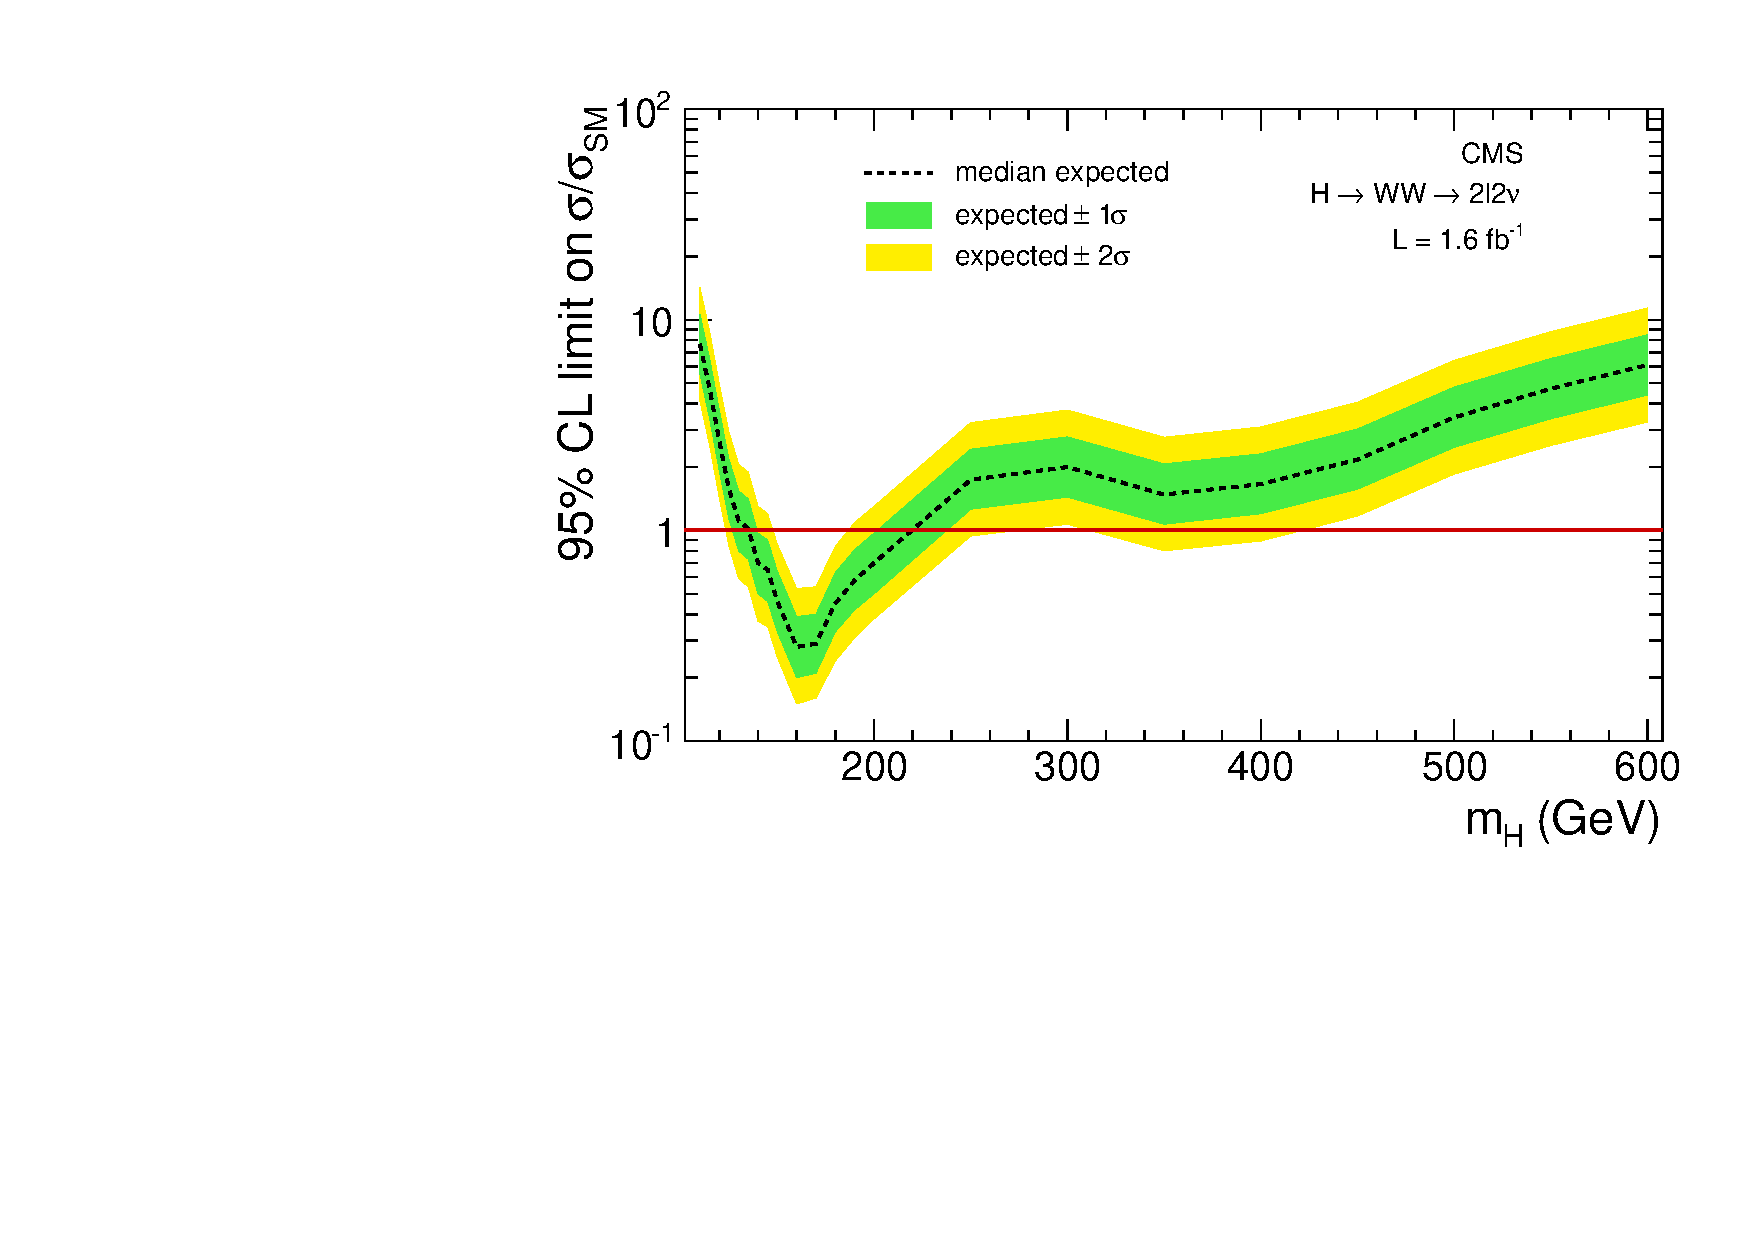
\includegraphics[width=.45\textwidth]{figures/limits_nj_cut_extended.pdf}
}
\subfigure[SM Higgs Zoomed (cut-based)]{
\centering
\label{subfig:sm_cut_zoom}
%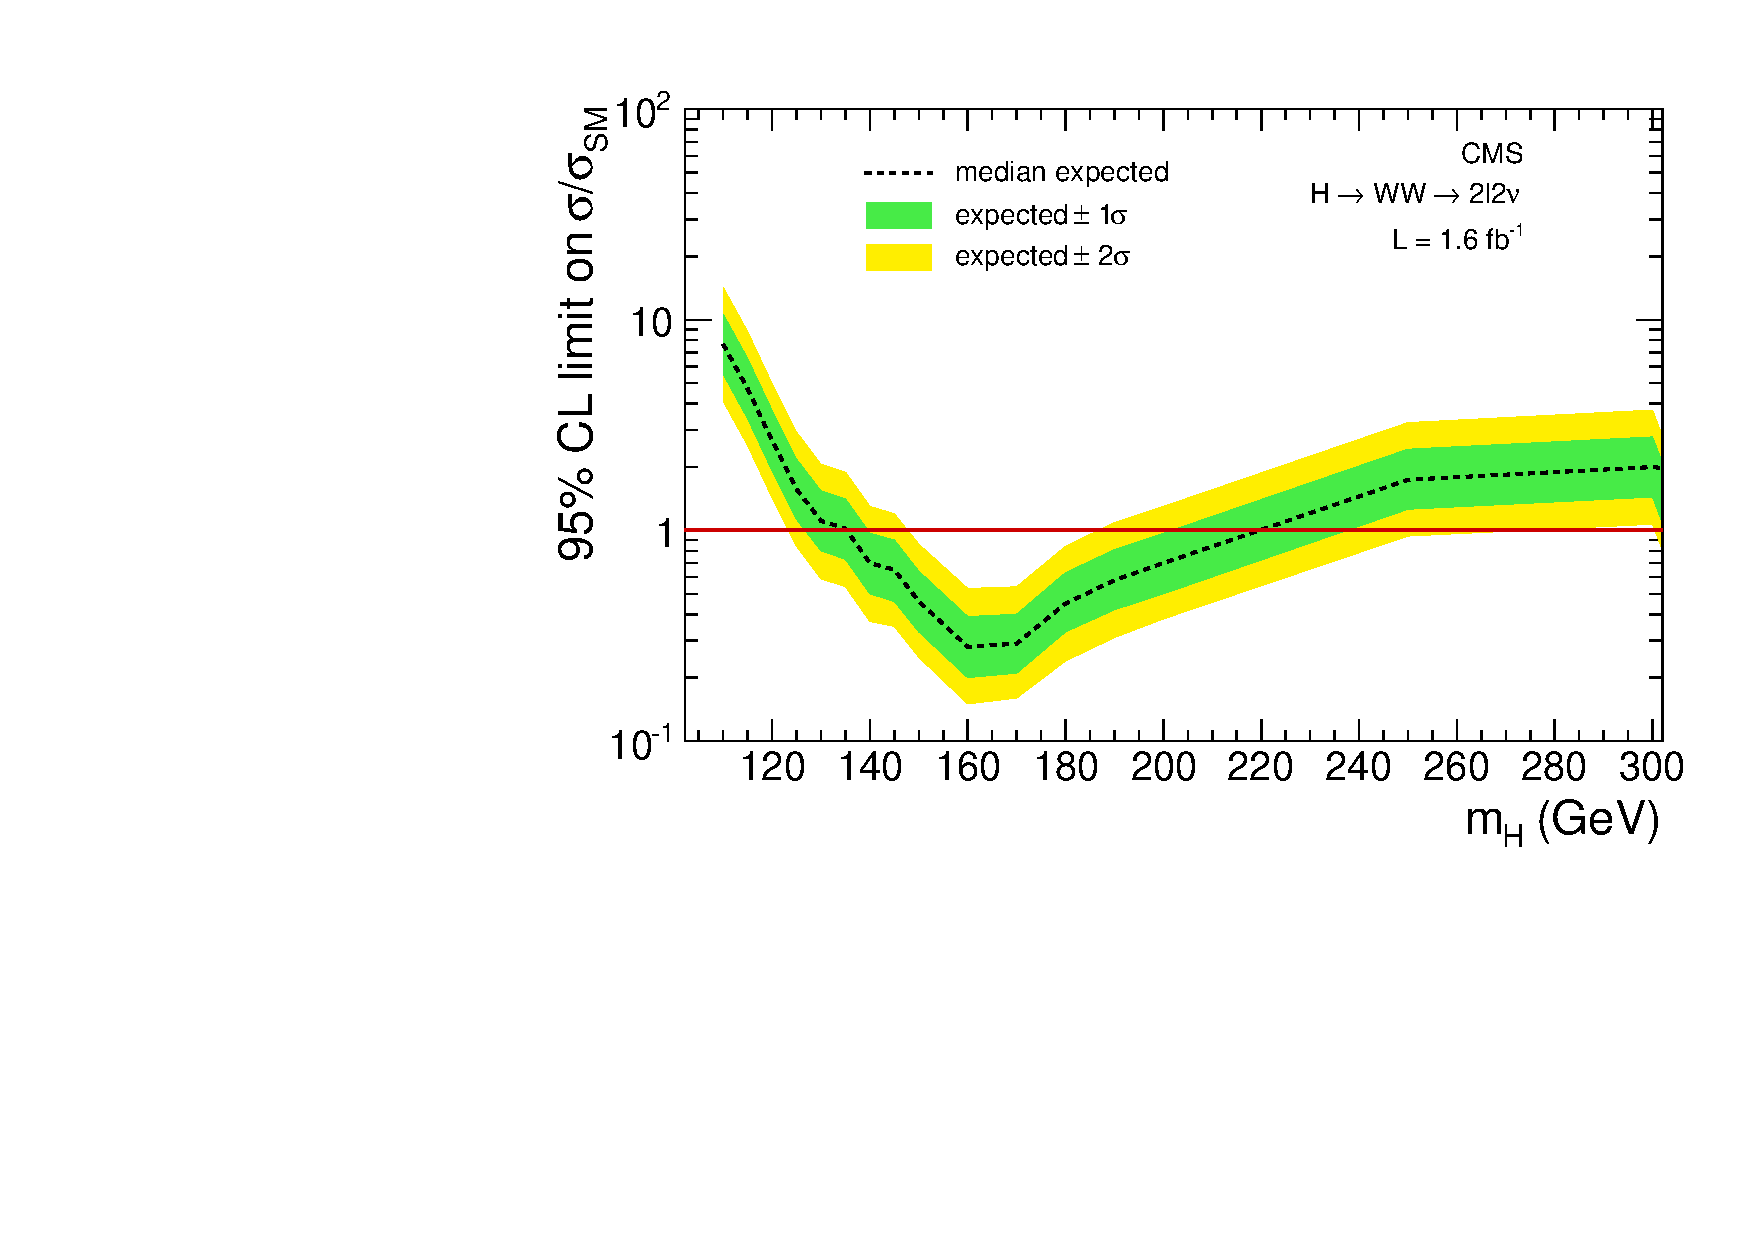
\includegraphics[width=.45\textwidth]{figures/limits_nj_cut.pdf}
}
\centering
\subfigure[SM Higgs (shape-based)]{
\centering
\label{subfig:sm_shape}
%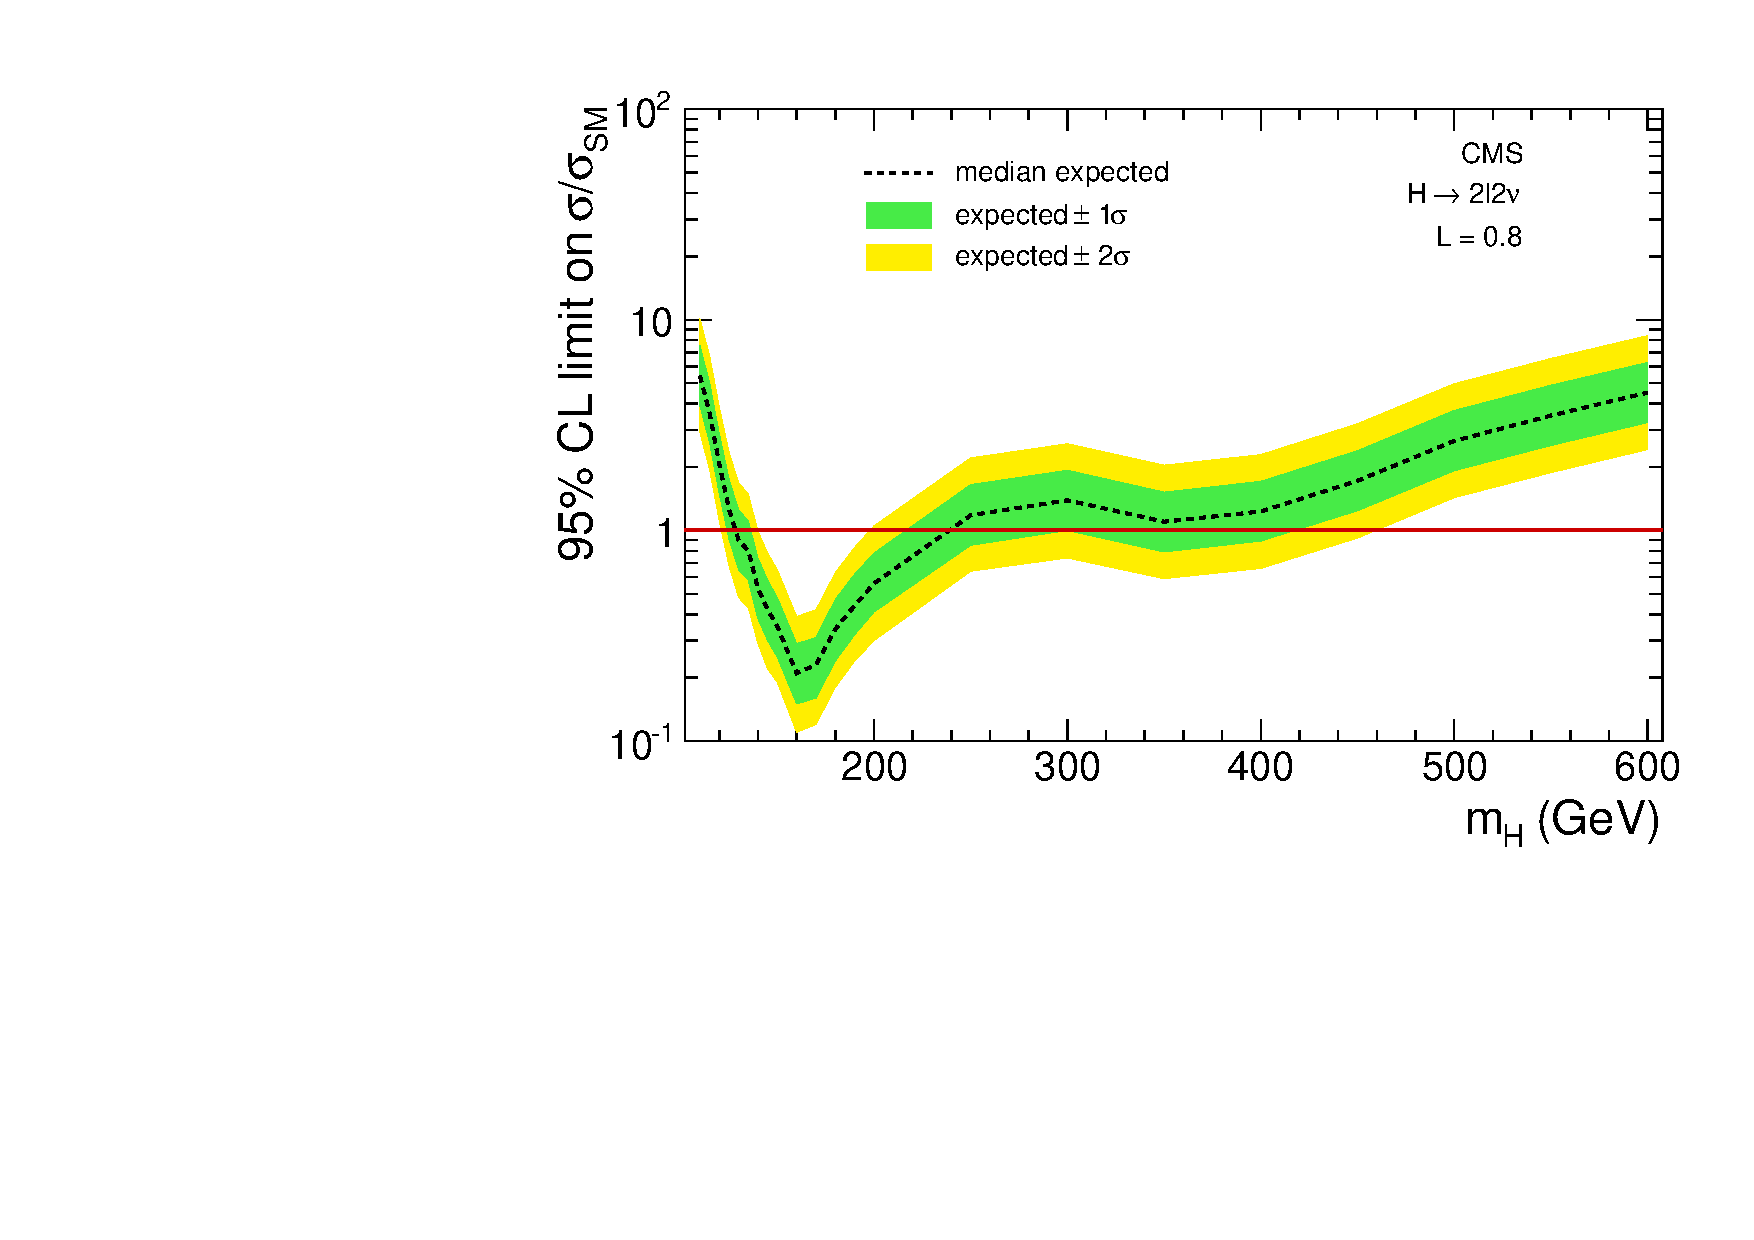
\includegraphics[width=.45\textwidth]{figures/limits_nj_shape_extended.pdf}
}
\subfigure[SM Higgs Zoomed (shape-based)]{
\centering
\label{subfig:sm_shape_zoom}
%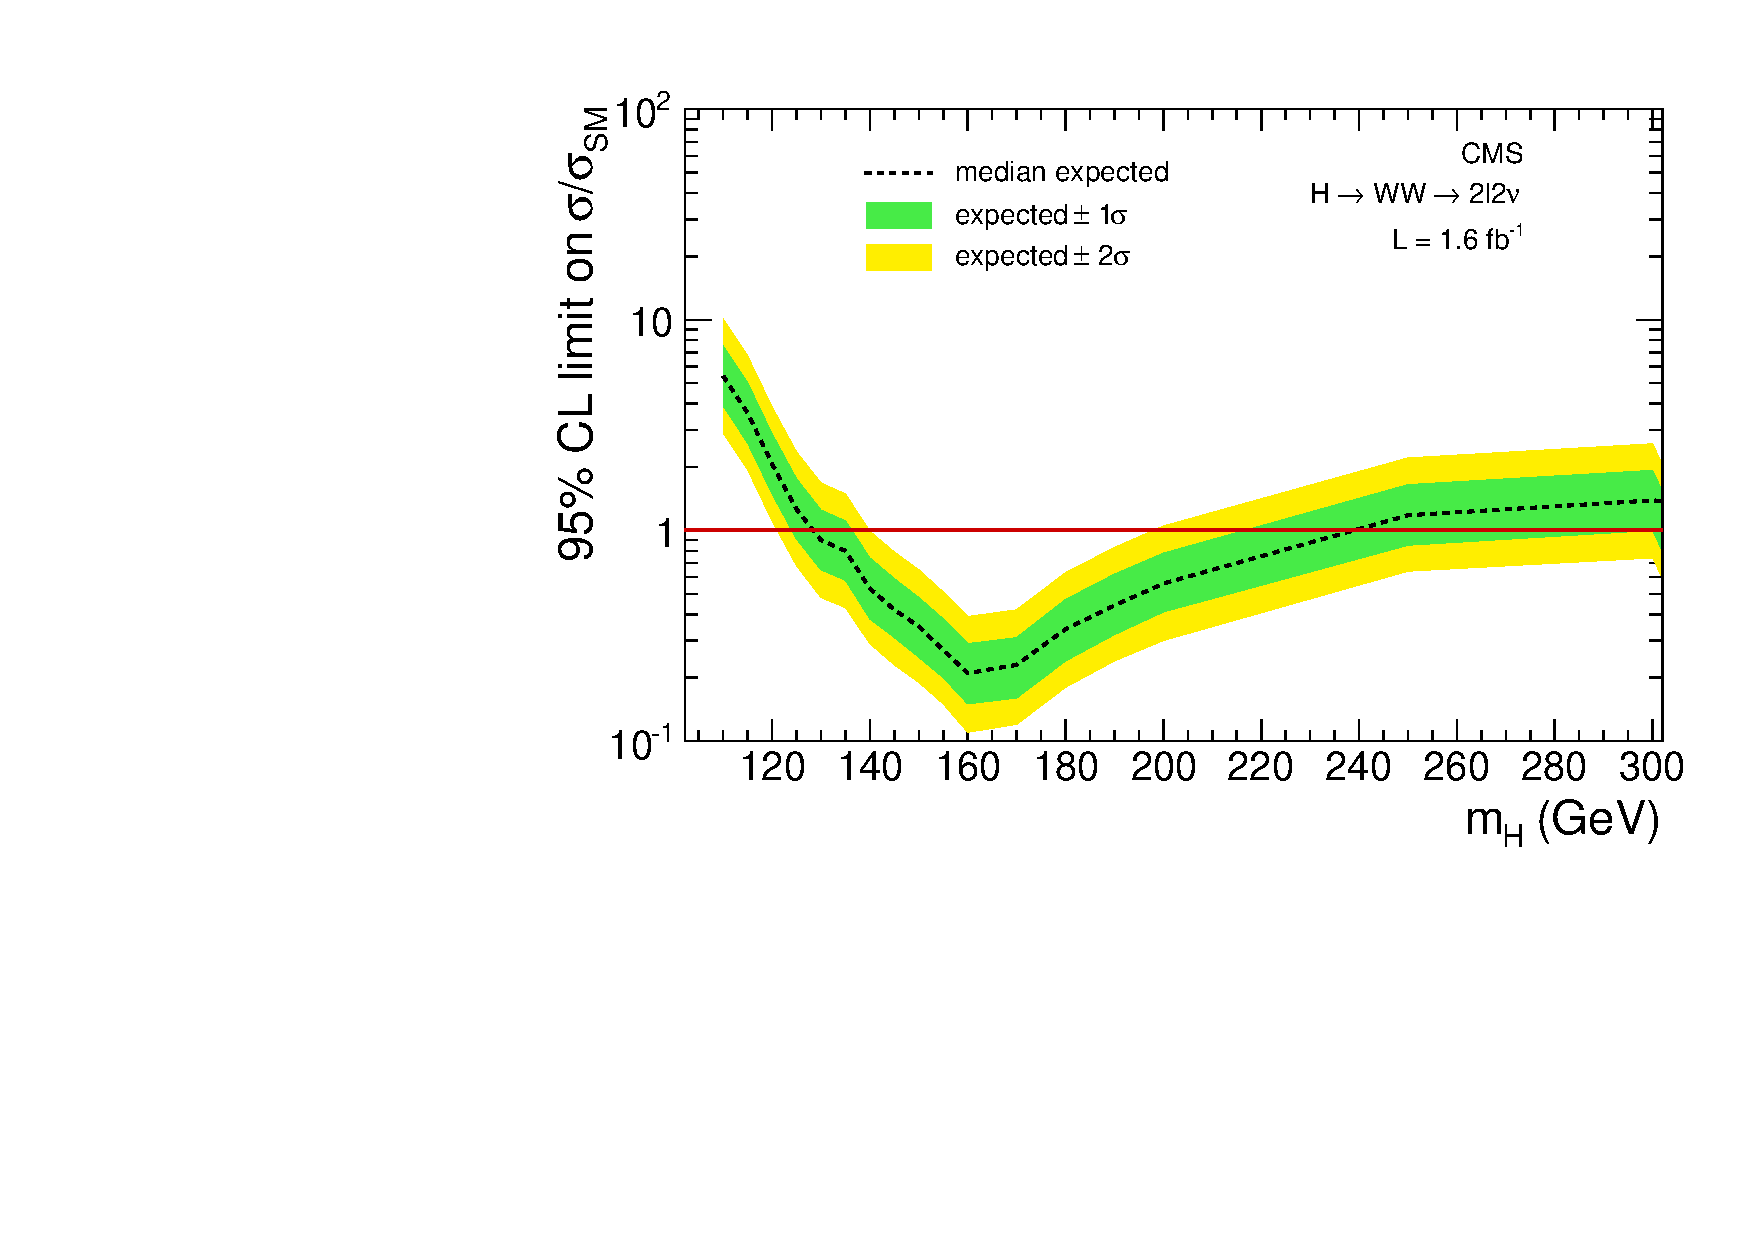
\includegraphics[width=.45\textwidth]{figures/limits_nj_shape.pdf}
}
\centering
\subfigure[Fermiophobic Higgs (cut-based)]{
\centering
\label{subfig:sm_fp}
%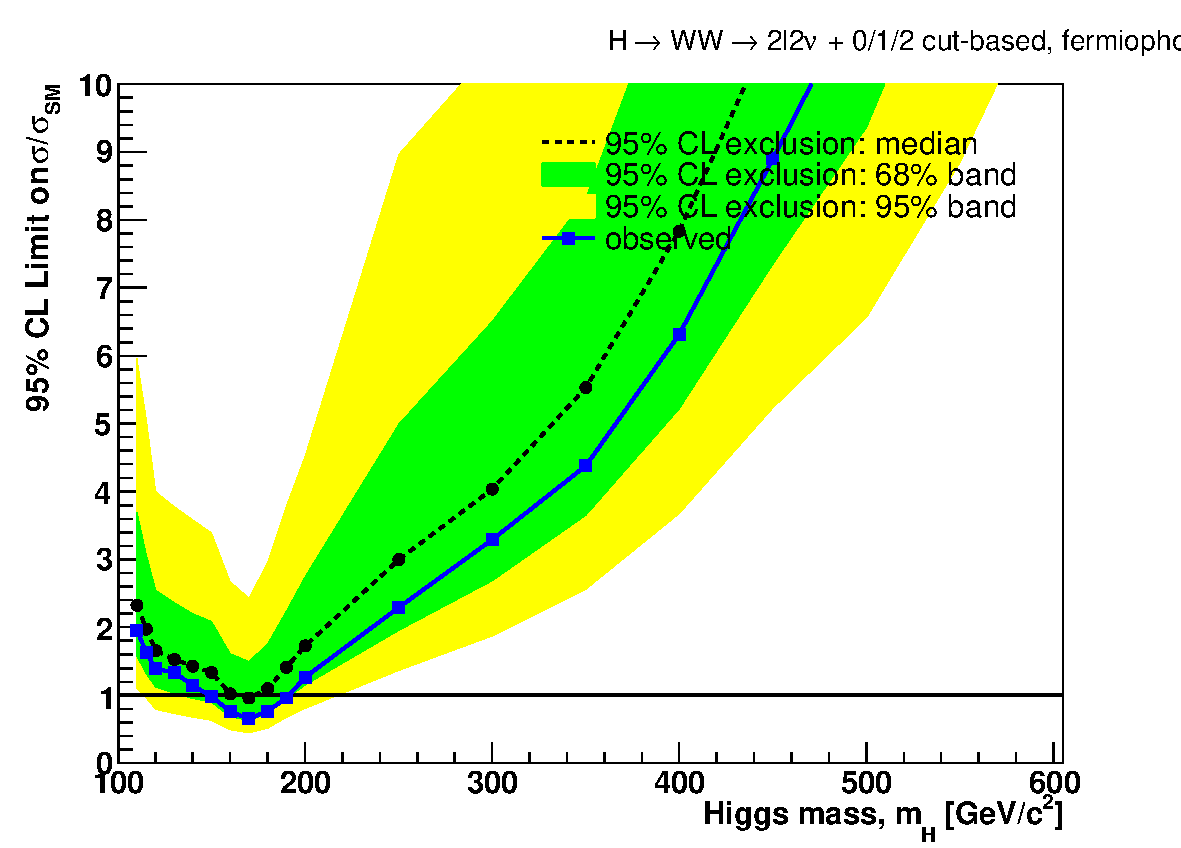
\includegraphics[width=.45\textwidth]{figures/limits_nj_cut_noggH_extended.pdf}
}
\subfigure[Fermiophobic Higgs Zoomed (cut-based)]{
\centering
\label{subfig:sm_fp_zoom}
%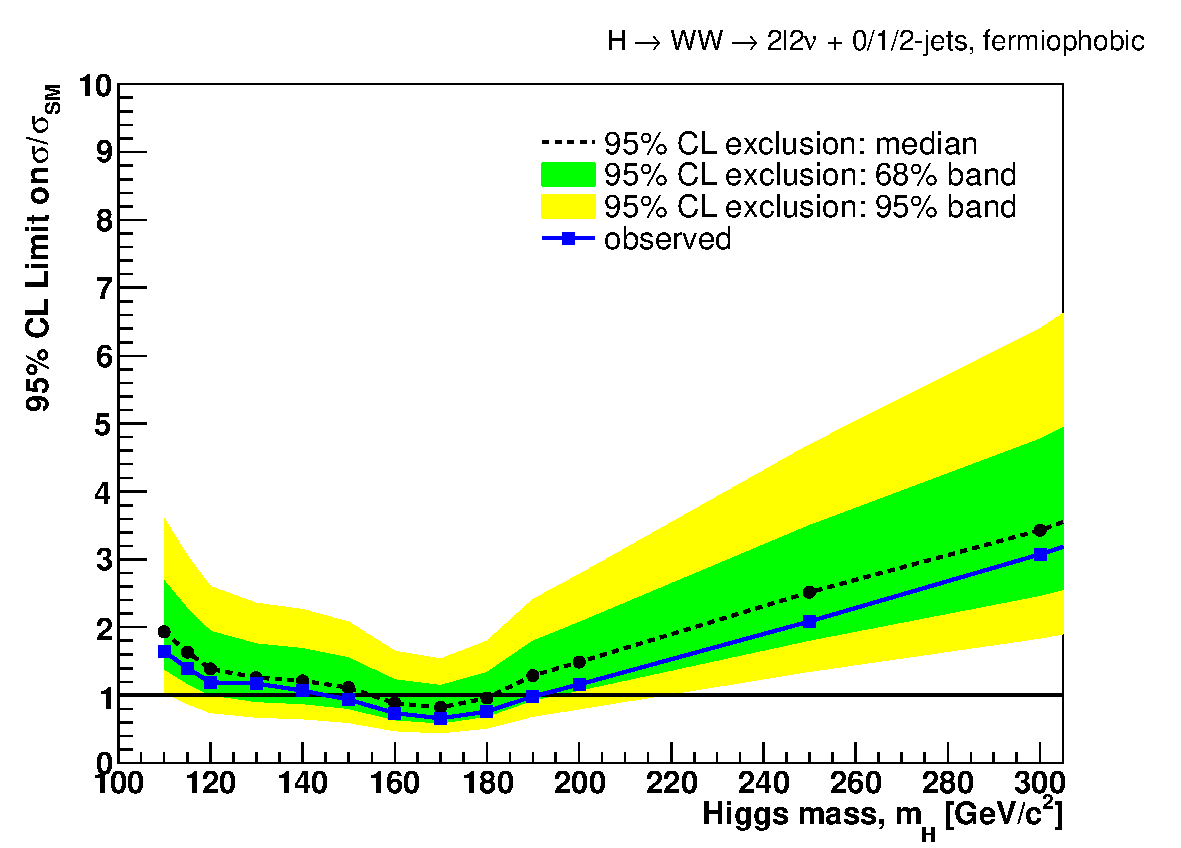
\includegraphics[width=.45\textwidth]{figures/limits_nj_cut_noggH.pdf}
} \\ 
\caption{Expected and observed upper limits on the Standard Model (SM)
  and Fermiophobic Higgs models.}
\label{fig:uls}
\end{figure}


%%%%%%%%%%%%%%%%%%%%%%%%%%%%%%
\begin{table}[hbp!]
\begin{center}
\begin{tabular}{c c c c c}
\hline
\vspace{-3mm} && \\
 Higgs Mass   & Observed & Median expected & Expected range for 68\% & Expected range for 95\%   \\
\vspace{-3mm} && \\
\hline
115 & 3.5 & 3.3 & [2.4, 4.5] & [1.8, 6.1] \\
120 & 2.1 & 1.9 & [1.4, 2.7] & [1.0, 3.6] \\
130 & 1.1 & 0.9 & [0.7, 1.3] & [0.5, 1.7] \\
140 & 0.6 & 0.6 & [0.4, 0.8] & [0.3, 1.1] \\
150 & 0.5 & 0.4 & [0.3, 0.6] & [0.2, 0.8] \\
160 & 0.3 & 0.2 & [0.2, 0.3] & [0.1, 0.5] \\
170 & 0.2 & 0.3 & [0.2, 0.4] & [0.1, 0.5] \\
180 & 0.3 & 0.3 & [0.2, 0.5] & [0.2, 0.6] \\
190 & 0.4 & 0.5 & [0.4, 0.7] & [0.3, 0.9] \\
200 & 0.6 & 0.6 & [0.4, 0.9] & [0.3, 1.2] \\
250 & 1.1 & 1.2 & [0.9, 1.7] & [0.6, 2.2] \\
300 & 1.7 & 1.4 & [1.0, 2.0] & [0.8, 2.6] \\
350 & 1.5 & 1.3 & [0.9, 1.8] & [0.7, 2.5] \\
400 & 1.7 & 1.5 & [1.0, 2.0] & [0.8, 2.7] \\
450 & 2.0 & 1.8 & [1.3, 2.5] & [1.0, 3.4] \\
500 & 2.5 & 2.5 & [1.8, 3.4] & [1.3, 4.6] \\
550 & 3.7 & 3.4 & [2.5, 4.8] & [1.8, 6.4] \\
600 & 5.1 & 4.9 & [3.5, 6.8] & [2.6, 9.1] \\
\hline
\end{tabular}
\caption{Expected and observed upper limits for SM Higgs using the
  {\bf cut-based} analysis with \intlumiEightTeV\ of data}
\label{tab:cutbase_uls}
\end{center}
\end{table}
%%%%%%%%%%%%%%%%%%%%%%%%%%%%%%

%%%%%%%%%%%%%%%%%%%%%%%%%%%%%%
\begin{table}[hbp!]
\begin{center}
\begin{tabular}{c c c c c}
\hline
\vspace{-3mm} && \\
 Higgs Mass   & Observed & Median expected & Expected range for 68\% & Expected range for 95\%   \\
\vspace{-3mm} && \\
\hline
110 & 7.9 & 5.3 & [3.8, 7.4] & [2.9, 9.9] \\
115 & 4.6 & 2.6 & [1.9, 3.6] & [1.4, 4.8] \\
120 & 2.4 & 1.5 & [1.1, 2.1] & [0.8, 2.8] \\
130 & 0.8 & 0.7 & [0.5, 1.0] & [0.4, 1.4] \\
140 & 0.6 & 0.4 & [0.3, 0.6] & [0.2, 0.8] \\
150 & 0.4 & 0.3 & [0.2, 0.4] & [0.2, 0.6] \\
160 & 0.2 & 0.2 & [0.1, 0.3] & [0.1, 0.3] \\
170 & 0.3 & 0.2 & [0.1, 0.3] & [0.1, 0.4] \\
180 & 0.3 & 0.3 & [0.2, 0.4] & [0.1, 0.5] \\
190 & 0.4 & 0.4 & [0.3, 0.5] & [0.2, 0.7] \\
200 & 0.5 & 0.5 & [0.4, 0.7] & [0.3, 0.9] \\
250 & 0.7 & 0.9 & [0.7, 1.3] & [0.5, 1.8] \\
300 & 1.1 & 1.0 & [0.8, 1.4] & [0.6, 1.9] \\
350 & 0.9 & 0.9 & [0.7, 1.3] & [0.5, 1.7] \\
400 & 1.3 & 1.0 & [0.7, 1.4] & [0.5, 1.8] \\
450 & 1.1 & 1.3 & [1.0, 1.8] & [0.7, 2.5] \\
500 & 1.3 & 1.9 & [1.3, 2.6] & [1.0, 3.5] \\
550 & 2.0 & 2.7 & [1.9, 3.7] & [1.4, 5.0] \\
600 & 2.4 & 3.8 & [2.8, 5.3] & [2.1, 7.2] \\
\hline
\end{tabular}
\caption{Expected and observed upper limits for SM Higgs using the
  {\bf shape-based} analysis with \intlumiEightTeV\ of data}
\label{tab:mvabase_uls}
\end{center}
\end{table}
%%%%%%%%%%%%%%%%%%%%%%%%%%%%%%

%%%%%%%%%%%%%%%%%%%%%%%%%%%%%%
\begin{table}[hbp!]
\begin{center}
\begin{tabular}{c c c c c}
\hline
\vspace{-3mm} && \\
 Higgs Mass   & Observed & Median expected & Expected range for 68\% & Expected range for 95\%   \\
\vspace{-3mm} && \\
\hline
110 & 1.7 & 1.9 & [1.4, 2.7] & [1.0, 3.6] \\
115 & 1.4 & 1.6 & [1.2, 2.3] & [0.9, 3.0] \\
120 & 1.2 & 1.4 & [1.0, 1.9] & [0.7, 2.6] \\
130 & 1.2 & 1.3 & [0.9, 1.8] & [0.7, 2.4] \\
140 & 1.1 & 1.2 & [0.9, 1.7] & [0.7, 2.3] \\
150 & 0.9 & 1.1 & [0.8, 1.6] & [0.6, 2.1] \\
160 & 0.7 & 0.9 & [0.6, 1.2] & [0.5, 1.7] \\
170 & 0.7 & 0.8 & [0.6, 1.1] & [0.4, 1.5] \\
180 & 0.8 & 1.0 & [0.7, 1.3] & [0.5, 1.8] \\
190 & 1.0 & 1.3 & [0.9, 1.8] & [0.7, 2.4] \\
200 & 1.2 & 1.5 & [1.1, 2.1] & [0.8, 2.8] \\
250 & 2.1 & 2.5 & [1.8, 3.5] & [1.3, 4.7] \\
300 & 3.1 & 3.4 & [2.5, 4.8] & [1.8, 6.4] \\
350 & 4.1 & 4.6 & [3.3, 6.4] & [2.5, 8.6] \\
400 & 5.9 & 6.7 & [4.8, 9.3] & [3.6, 12.4] \\
450 & 8.2 & 9.5 & [6.8, 13.2] & [5.1, 17.6] \\
500 & 10.7 & 12.2 & [8.8, 17.0] & [6.6, 22.8] \\
550 & 13.2 & 15.9 & [11.4, 22.1] & [8.5, 29.6] \\
600 & 16.8 & 20.4 & [14.7, 28.3] & [10.9, 38.0] \\
\hline
\end{tabular}
\caption{Expected and observed upper limits for {\bf the fermiophobic
    Higgs boson hypothesis} using the cut-based analysis with
  \intlumiEightTeV\ of data}
\label{tab:cutbase_uls_fp}
\end{center}
\end{table}
%%%%%%%%%%%%%%%%%%%%%%%%%%%%%%
